\documentclass[11pt]{article}
\usepackage[T1]{fontenc}
\usepackage[utf8]{inputenc}
\usepackage{lmodern}
\usepackage[margin=1.1in]{geometry}
\usepackage{amsmath,amssymb,amsthm,mathtools}
\usepackage{microtype}
\usepackage{xcolor}
\usepackage{enumitem}
\usepackage{booktabs}
\usepackage{flafter}
\usepackage{tikz}
\usetikzlibrary{arrows.meta,positioning,calc,fit}
\usepackage{tikz-cd}
\usepackage{hyperref}
\usepackage[capitalise,noabbrev,nameinlink]{cleveref}
\hypersetup{
  colorlinks=true,
  linkcolor=blue!35!black,
  citecolor=green!30!black,
  urlcolor=blue!50!black,
  pdftitle={The Hilbert--Smith conjecture in every finite dimension},
  pdfauthor={OpenAI},
  pdfsubject={Continuous transformation groups and the Hilbert--Smith conjecture}
}
\numberwithin{equation}{section}
\newtheorem{theorem}{Theorem}[section]
\newtheorem{lemma}[theorem]{Lemma}
\newtheorem{proposition}[theorem]{Proposition}
\newtheorem{corollary}[theorem]{Corollary}
\theoremstyle{definition}
\newtheorem{definition}[theorem]{Definition}
\newtheorem{convention}[theorem]{Convention}
\newtheorem{notation}[theorem]{Notation}
\theoremstyle{remark}
\newtheorem{remark}[theorem]{Remark}
\crefname{theorem}{Theorem}{Theorems}
\crefname{lemma}{Lemma}{Lemmas}
\crefname{proposition}{Proposition}{Propositions}
\crefname{corollary}{Corollary}{Corollaries}
\crefname{definition}{Definition}{Definitions}
\crefname{remark}{Remark}{Remarks}
\crefname{section}{Section}{Sections}
\crefname{equation}{Equation}{Equations}
\crefname{figure}{Figure}{Figures}
\newcommand{\R}{\mathbb R}
\newcommand{\C}{\mathbb C}
\newcommand{\Q}{\mathbb Q}
\newcommand{\Z}{\mathbb Z}
\newcommand{\Zp}{\mathbb Z_p}
\newcommand{\D}{\mathcal D}
\newcommand{\T}{\mathcal T}
\newcommand{\Tzero}{\mathcal T^0}
\newcommand{\Pcat}{\mathcal P}
\newcommand{\Pzero}{\mathcal P^0}
\newcommand{\Bcat}{\mathcal B}
\newcommand{\Bzero}{\mathcal B^0}
\newcommand{\const}[2]{\underline{#1}_{#2}}
\newcommand{\pt}{\mathrm{pt}}
\newcommand{\id}{\mathrm{id}}
\newcommand{\HH}{\mathbb H}
\newcommand{\Witt}{W}
\DeclareMathOperator{\Hom}{Hom}
\DeclareMathOperator{\supp}{supp}
\DeclareMathOperator{\im}{im}
\DeclareMathOperator{\coker}{coker}
\DeclareMathOperator{\rk}{rank}
\DeclareMathOperator{\sgn}{sign}
\DeclareMathOperator{\Cone}{Cone}
\DeclareMathOperator{\Homeo}{Homeo}
\DeclareMathOperator{\Fix}{Fix}
\DeclareMathOperator{\intt}{int}
\DeclareMathOperator{\Tr}{Tr}
\DeclareMathOperator{\colim}{colim}
\setlist{topsep=5pt,itemsep=3pt,parsep=0pt}
\setlength{\emergencystretch}{1em}
\allowdisplaybreaks[1]
\title{The Hilbert--Smith conjecture in every finite dimension}
\author{OpenAI}
\date{September 23, 2026}
\makeatletter
\renewcommand{\maketitle}{%
  \begin{center}{\LARGE\@title\par}\vspace{1em}{\large\@author\par}\vspace{.5em}{\@date\par}\end{center}
  \vspace{.5em}%
}
\makeatother
\begin{document}
\maketitle
\begin{abstract}
We prove the Hilbert--Smith conjecture in every finite dimension: every
locally compact second-countable Hausdorff group acting faithfully and
jointly continuously on a connected Hausdorff second-countable
finite-dimensional topological manifold without boundary is a Lie group.
\end{abstract}
\begingroup
\small
\setlength{\baselineskip}{0.92\baselineskip}
\tableofcontents
\endgroup
\clearpage
\section{Introduction}\label{sec:introduction}

The Hilbert--Smith conjecture asks whether a locally compact group acting
faithfully and continuously on a connected topological manifold must be
a Lie group. An action is \emph{faithful} when its kernel is trivial:
no nonidentity element fixes every point. Faithfulness does not require
point stabilizers to be trivial. We prove the following statement.

\begin{theorem}[The Hilbert--Smith conjecture]\label{cor:lie}
Let \(n\geq1\). A locally compact second-countable Hausdorff group
acting faithfully and jointly continuously on a connected Hausdorff
second-countable topological \(n\)-manifold without boundary is a Lie
group.
\end{theorem}

This gives a positive resolution in every positive finite dimension.
The manifold may be noncompact, nonorientable, or nontriangulable;
fixed points and arbitrary stabilizers are allowed. In dimension zero,
a connected manifold is a point, so a faithful acting group is trivial
and the conclusion holds as well.

The mechanism is the exclusion of faithful actions of the additive
group of \(p\)-adic integers, for a prime \(p\),
\[
  \Zp=\varprojlim_k\Z/p^k\Z,
\]
with its profinite topology. The precise classical reduction from the
full group theorem to this case is recalled at the end of the proof.

\begin{theorem}[$p$-adic exclusion]\label{thm:main}
Let \(n\geq1\) be an integer and \(p\) a prime. Every jointly continuous
action of \(\Zp\) on a connected Hausdorff second-countable topological
\(n\)-manifold without boundary has nonzero kernel. Consequently the
action factors through a finite quotient of \(\Zp\).
\end{theorem}

For a manifold \(M\), equip \(\Homeo(M)\) with the compact-open
topology. Jointly continuous
actions are equivalently continuous homomorphisms
\(\Zp\to\Homeo(M)\). No dimension bound on the orbit space is assumed.

\Cref{cor:lie} also gives the dynamical consequence recorded in
\cite[Conjecture~1.4]{Pardon2013}. For a manifold $M$ as in
\Cref{cor:lie}, a homeomorphism $f$ is \emph{almost periodic} if the
cyclic subgroup $\{f^j:j\in\Z\}$ has compact closure $K$ in
$\Homeo(M)$. Some positive iterate of $f$ is then the time-one map
of a continuous real flow: there are an integer $m\geq1$ and a
continuous homomorphism $\Phi:\R\to\Homeo(M)$ with
$\Phi(1)=f^m$. Indeed, $K$ is a compact abelian group acting faithfully
and jointly continuously on $M$. Evaluation on a countable dense
subset of $M$ embeds $K$ into a countable product of copies of $M$,
so $K$ is second countable. By \Cref{cor:lie}, it is a compact abelian
Lie group. Its identity component $K^0$ is a torus of finite index,
so $f^m\in K^0$ for some $m\geq1$. The surjective exponential map
of this torus places $f^m$ on a one-parameter subgroup, giving $\Phi$.

\subsection{The problem and its predecessors}

Hilbert's fifth problem asked how far differentiability assumptions
could be removed from the theory of continuous transformation groups
\cite[Problem~5]{Hilbert1902}.
One central formulation concerns a group that is itself locally
Euclidean. Gleason and Montgomery--Zippin resolved that formulation in
1952 \cite{Gleason1952,MontgomeryZippin1952}, and Yamabe extended the
structure theory to general locally compact groups
\cite{Yamabe1953a,Yamabe1953b}.
Hilbert--Smith asks for the restrictions imposed by a faithful action
on a connected manifold. The passage to additive $p$-adic groups
combines this structure theory with rigidity of periodic
transformations. Lee gives a treatment of the reduction
\cite{Lee1997}; Pardon's introduction states the action-specific form
used here \cite[Introduction, p.~1]{Pardon2013}. The structure theory is
developed systematically in Montgomery--Zippin
\cite{MontgomeryZippin1955}.

The low-dimensional cases illustrate how much geometry may be needed to
control a merely continuous action.  The cases of one- and two-manifolds
were classical; Pardon gives a later account and proof of the
two-dimensional case, crediting Montgomery--Zippin
\cite{Pardon2019}.  Pardon proved the three-dimensional conjecture
\cite[Theorem~1.5]{Pardon2013}.  His local argument uses incompressible
surfaces in a suitable invariant open set and the resulting action on a
surface mapping class group.  In particular, it accommodates arbitrary
stabilizers without replacing the given action by a smooth action.

Another line of work controls the action by its regularity.
Bochner--Montgomery established the differentiable precedent
\cite{BochnerMontgomery1946}.
Repov\v{s}--\v{S}\v{c}epin proved the Lipschitz case on Riemannian
manifolds \cite[Theorem~1.1]{RepovsScepin1997}, and Maleshich obtained
an obstruction for H\"older actions on closed manifolds when a common
exponent exceeds $n/(n+2)$ \cite[Theorem~3.1]{Maleshich1997}.
Martin established the quasiconformal case on Riemannian manifolds
\cite[Theorems~1.2--1.3]{Martin1999}.
These results impose regularity on the transformations, rather than only
on the underlying manifold.

The metric arguments connect to the dimension-raising theory of
Yang and Bredon--Raymond--Williams
\cite{Yang1960,BredonRaymondWilliams1961}.
Their obstruction concerns integral cohomological dimension;
Raymond's subsequent analysis emphasizes the different behavior with
field coefficients \cite{Raymond1961}.
In the Lipschitz proof, an averaged invariant metric keeps Hausdorff
dimension small enough to contradict the required dimension increase
of the orbit space.
Mj extended this approach to uniformly quasisymmetric actions on
compact metric cohomology manifolds under Ahlfors regularity and
Hausdorff-dimension hypotheses, with applications to boundaries of
Poincar\'e duality hyperbolic groups
\cite[Theorem~2.24 and Corollary~2.25]{Mj2012}.

Shelukhin used Floer-theoretic methods to exclude nontrivial continuous
$p$-adic actions by homeomorphisms in the $C^0$-closure of the Hamiltonian
diffeomorphism group of a closed symplectic manifold on whose $\pi_2$
both the symplectic class and the first Chern class vanish
\cite[Theorem~A]{Shelukhin2024}.

Newman's rigidity theorem for periodic transformations
\cite{Newman1931} supplies the local input used here: a finite-order
homeomorphism of a connected manifold that fixes a nonempty open set
pointwise is the identity. For a modern statement and proof, see
\cite[author manuscript, pp.~2--3]{Pardon2019}.
Pardon's local reduction \cite[\S4.1]{Pardon2013} uses this rigidity to
find a faithful action of an open subgroup on an invariant open subset
of one coordinate chart. We use that reduction without imposing
regularity on the transformations or on the boundary of the chart subset.

\subsection{Duality and signatures}

The signature viewpoint has a separate line of antecedents.
Verdier developed duality for sheaves on locally compact spaces
\cite{Verdier1966}; we use its derived functor formulation in
Kashiwara--Schapira and Schapira
\cite{KashiwaraSchapira1990,SchapiraNotes}.
Balmer's triangular Witt groups package symmetric forms and their
neutral relations in categories with duality \cite{Balmer2000}.
For localization we use Balmer--Walter's published
Theorem~2.1, which removes the weak-cancellation hypothesis of the
earlier localization theorem \cite{BalmerWalter2002}.
Woolf applied this formalism both to perfect complexes of sheaves and
to constructible complexes. Using duality on perfect complexes, he
proved a cylinder homotopy relation for that theory and obtained a
generalized homology theory from constructible Witt groups on compact
polyhedra
\cite{Woolf2008}.
Ranicki--Weiss construct rational Pontryagin classes using a local
chain theory generated by continuous simplex maps, with cutoff by
subdivision, excision, and control of passage to direct summands
\cite[\S4 and Theorems~8.2--8.3]{RanickiWeiss2010}.
Their chain-level $L$-theory differs from the sheaf Witt groups used
here, but its generated-category strategy is a close antecedent.

Our categories are generated by proper images of finite polyhedra under
arbitrary continuous maps. Such images need not be constructible.
We verify that duality and the constructions in the cylinder relation
restrict to these specified generated categories. The additional
quotient comparison and uniform integral bound establish the fixed
signature lattice.
The comparison is integral before rationalization: a rational
isomorphism alone would not bound the possible denominators.

\subsection{The obstruction: equal parts in a fixed lattice}

The numerical contradiction is simple. Fix an odd integer
\(d\geq3\); for an action on an \(n\)-manifold, we will take \(d>n\).
We construct an abelian group \(E_d(S^d)\), an orientation
class \(u_d\), and a positive integer \(L_d\). For an integral class
\(x\), write \(\overline{x}=x\otimes1\) for its rational image. Then
\begin{equation}\label{intro:lattice}
 E_d(S^d)\otimes\Q=\Q\overline{u}_d,
 \qquad
 \im\bigl(E_d(S^d)\to E_d(S^d)\otimes\Q\bigr)
       \subseteq L_d^{-1}\Z\overline{u}_d.
\end{equation}
A faithful \(\Zp\)-action will produce, for every \(k\geq1\),
\(p^k\) integral classes in this group. Their rational images are equal
and sum to \(4\overline{u}_d\). Each image is therefore
\((4/p^k)\overline{u}_d\), which
contradicts \Cref{intro:lattice} as soon as \(p^k>4L_d\).
The order of these choices matters: \(L_d\) is fixed before \(k\).

Here ``integral'' refers to an element of the abelian Witt group before
it is tensored with \(\Q\); the sheaf coefficients are real throughout.
For a map from a compact polyhedron, its direct-image sheaf complex
records the cohomology of the fibers. A symmetric self-duality on that
complex supplies signature data, and the Witt group sets forms with
a lagrangian equal to zero. This makes the invariant additive
while retaining the integrality of ordinary signature.

Here is the group underlying this argument. For a finite polyhedron \(X\), let
\(\T(X)\) be the full thick subcategory of the bounded derived category
of real sheaves generated by
\[
 Rf_*\const{\R}{B},\qquad f:B\longrightarrow X,
 \qquad B\text{ a compact finite polyhedron},
\]
where \(f\) is continuous. Thus an object is obtained by finite sums,
shifts, cones, and direct summands from these proper direct images.
Their stalks need not be finite dimensional. Verdier duality nevertheless
restricts to this category, as we prove from simplex generators.
We put \(E_r(X)=W_r(\T(X))\), the Witt group of nonsingular symmetric
forms for the shifted duality \(\D_{X,r}=[-r]\D_X\), with neutral forms
set equal to zero. \Cref{sec:categories} gives the precise definitions,
the signs, and homotopy invariance.

To establish \Cref{intro:lattice}, we compare with the subcategory
generated by semialgebraic maps. On a suitably chosen oriented ball,
finite Witt relations can be evaluated by ordinary integral signature. Two
arguments transfer that integrality to the continuous category.
First, cutting off the finite polyhedral sources identifies quotient
morphisms with germs near a closed set. Second, a full dense
triangulated inclusion with duality, in which every object of the larger
category is a summand of one from the smaller category, admits a map
on Witt groups in
the reverse direction whose two composites are multiplication by
\(2\). The resulting exponent-two kernel and cokernel bound is a
consequence of Hornbostel--Schlichting's cofinality theorem
\cite[author preprint, Appendix~A, Theorem~A.2]{HornbostelSchlichting2004}.
We give the cutoff and explicit doubling constructions in
\Cref{sec:localization}; neither requires the images of arbitrary
continuous maps to be constructible.

Localization on a finite cover of the sphere then bounds both the
kernel and the cokernel of comparison by a fixed power of \(2\), in
every degree. This proves the lattice statement in
\Cref{thm:sphere-lattice}. Rational equivalence alone would lose the
denominator bound. The cutoff description and the integral bound for
dense inclusions are also useful independently of the group action;
they supply the additional comparison needed beyond the constructible
homology theory of \cite{Woolf2008}.

\subsection{How the action supplies the equal parts}

Suppose that a faithful action exists on an \(n\)-manifold. By Newman's
theorem, a small open subgroup \(G\cong\Zp\) acts faithfully and
preserves orientation on a connected invariant open subset
\(O\subset\R^n\) of one coordinate chart. Choose an odd integer
\(d>n\), with \(d\geq3\), and give
\[
 W=O\times\R^{d-n}\subset\R^d
\]
the product action, trivial in the added coordinates. We use the
one-point compactification \(W^+\), its orbit space \(Y=W^+/G\),
and the maps
\[
 S^d\xrightarrow{c}W^+\xrightarrow{q}Y\xrightarrow{t}X.
\]
Here \(c\) collapses \(S^d\setminus W\) to \(\infty\), and \(t\)
is a continuous map into a compact space \(X\) homeomorphic to a finite
polyhedron. We require the value
\(b=tq(\infty)\) to have a basis of contractible open neighborhoods
in \(X\). The composite \(tqc\) always has the same finite-polyhedron
source \(S^d\), as shown in \Cref{fig:local-test}.

\begin{figure}[!htbp]
\centering
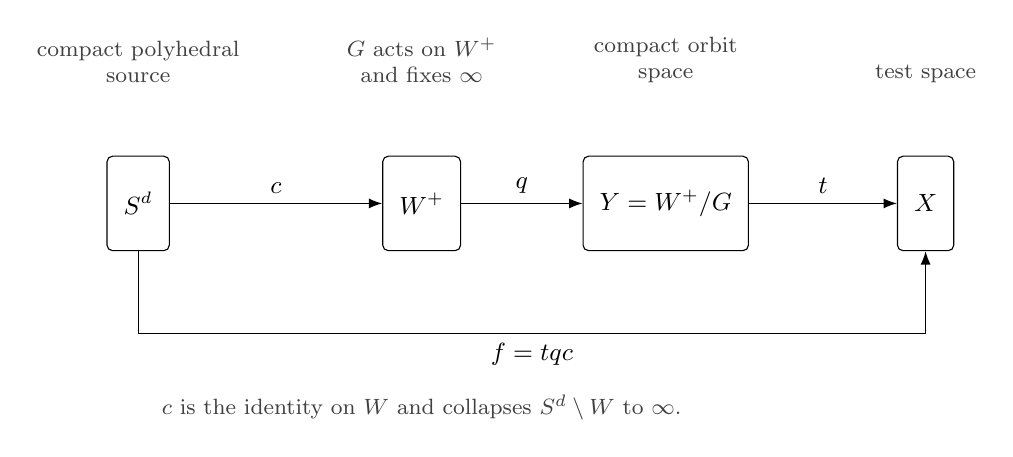
\begin{tikzpicture}[
  >=Latex,
  every node/.style={font=\small},
  space/.style={draw,rounded corners=2pt,align=center,
    minimum height=12mm,inner sep=6pt},
  note/.style={font=\footnotesize,align=center,text=black!75}
]
\node[space] (source) at (0,0) {\(S^d\)};
\node[space] (compact) at (3.6,0) {\(W^+\)};
\node[space] (orbit) at (6.7,0) {\(Y=W^+/G\)};
\node[space] (test) at (10.0,0) {\(X\)};
\draw[->] (source) -- node[above]{\(c\)} (compact);
\draw[->] (compact) -- node[above]{\(q\)} (orbit);
\draw[->] (orbit) -- node[above]{\(t\)} (test);
\draw[->] (source.south) -- ++(0,-1.05)
  -| node[pos=.25,below]{\(f=tqc\)} (test.south);
\node[note,above=8mm of source] {compact polyhedral\\source};
\node[note,above=8mm of compact] {\(G\) acts on \(W^+\)\\and fixes \(\infty\)};
\node[note,above=8mm of orbit] {compact orbit\\space};
\node[note,above=8mm of test] {test space};
\node[note,below=17mm of compact] {
  \(c\) is the identity on \(W\) and collapses \(S^d\setminus W\) to \(\infty\).};
\end{tikzpicture}
\caption{A local action produces compact-source tests. Away from
\(b=tq(\infty)\), the source of \(f\) lies in the oriented manifold
\(W=O\times\R^{d-n}\). The restricted map
\(f^{-1}(X\setminus\{b\})\to X\setminus\{b\}\) is proper, with oriented
manifold source.}
\label{fig:local-test}
\end{figure}


Put \(f_t=tqc\) and \(A_t=Rf_{t*}\const{\C}{S^d}\).
Here \(\C\) is the positive real plane with pairing
\(B(z,w)=\operatorname{Re}(z\overline w)\). Pushing this coefficient
pairing together with the orientation of \(S^d\) gives the degree-\(d\)
form \(\alpha_t\) on \(A_t\).
Away from \(b\), the map \(f_t\) is proper from an oriented open
subset of \(W\). Identify the characters of \(G\) with the group
\(\Lambda=\bigcup_{j\geq0}\mu_{p^j}\) of roots of unity of $p$-power
order. A finite partition \(\Lambda=D_0\sqcup\cdots\sqcup D_{m-1}\)
gives orthogonal projectors \(e_i\) on
\(A_t|_{X\setminus\{b\}}\) onto the corresponding character parts.
A projector need not extend to a summand over \(b\). Choose a
contractible open neighborhood \(U\) of \(b\). The projector's germ near
\(X\setminus U\) defines an endomorphism of \(A_t\) in the quotient
by objects compactly supported in \(U\).

For a self-adjoint projector \(e_i\), the operator \(2e_i-1\) is a
self-adjoint involution. We therefore have the following sum of forms
on the existing object:
\[
 [A_t,\alpha_t]+[A_t,\alpha_t(2e_i-1)].
\]
An integral localization
isomorphism lifts it to a class \(z_i(t)\in E_d(X)\). An explicit
matrix isometry gives
\(\sum_i z_i(t)=2[A_t,\alpha_t]\), without taking the images of
quotient idempotents.

Averaging a map supported in a ball gives a test \(a:Y\to S^d\)
with \(\deg(aqc)=1\). For each \(k\), faithfulness gives a nonempty
open region \(V\subset W/G\) over which
\(W/(p^kG)\to W/G\) consists of \(p^k\) labeled sheets.
Serre's results on odd spheres provide a map \(D_s:S^d\to S^d\)
of degree \(s>0\) such that \(D_s a\) is homotopic to a map constant
outside \(V\) \cite{Serre1951,Serre1953}. There a locally constant coefficient
isometry permutes \(p^k\) chosen character parts cyclically.
Covariance and homotopy invariance equate the rational images
\(s\overline{z}_i(a)\). Cancelling the nonzero rational scalar \(s\)
equates the \(\overline{z}_i(a)\), while the original integral classes
stay in the same fixed lattice. Their rational images sum to
\(4\overline{u}_d\): one factor of \(2\) comes from the real coefficient
plane and the other from the involution construction. The fixed lattice
gives the contradiction.

Only the actual manifold sources and the test spaces carry Verdier
duality in this argument. The compact orbit spaces enter through
ordinary sheaf direct images, averaging, and \v{C}ech cohomology.
No dimension bound on the orbit spaces or regularity assumption on
the boundary of \(O\) is used.
The odd stabilization is the only dimensional choice. In particular,
the proof treats both odd congruence classes of \(d\) modulo \(4\).

\Cref{sec:categories,sec:localization,sec:lattice} construct and bound
the signature invariant. \Cref{sec:local-tests} prepares the local
tests, including the odd-sphere argument. \Cref{sec:characters}
constructs the integral character classes and proves
\Cref{thm:main,cor:lie}.

\section{Compact-source sheaf categories and homotopy invariance}
\label{sec:categories}

The sheaves used below can have very complicated stalks.  Their finiteness
comes from their sources: they are built, by finitely many operations, from
proper images of constant sheaves on finite polyhedra.  We first establish
duality on exactly these categories, and then prove the cylinder relation
that will make their Witt groups homotopy invariant.

\subsection{Spaces, coefficients, and generators}

All sheaves in this section have coefficients in the field $\R$, regarded
algebraically.  A \emph{test space} is a locally compact, finite-dimensional,
separable metrizable space of the following kinds: a finite polyhedron, a
space homeomorphic to one, an open subset of such a space, or a finite
product of these spaces.  Points and the empty space are included.  The
spaces to which Verdier duality is applied will always be test spaces.

Write
\[
 \mathsf D(X)=D^b(\operatorname{Sh}_{\R}(X)).
\]
For a complex $A$, the assertion that its support is contained in a compact
set $K\subset X$ means that all its cohomology sheaves vanish on $X\setminus
K$.  We use this formulation even when the set of points with a nonzero
cohomology stalk is not closed.  All tensor products are derived tensor
products over $\R$; tensoring sheaves is exact over this field.

\begin{definition}[The test categories]
\label{def:test-categories}
Let $\Tzero(X)$ be the smallest full replete triangulated subcategory of
$\mathsf D(X)$ containing
\begin{equation}
 \label{cat:generators}
 Rf_*\const{\R}{B},
 \qquad f:B\longrightarrow X,
 \qquad B\text{ a compact finite polyhedron},
\end{equation}
where $f$ is any continuous map.  Let $\T(X)$ be its closure under direct
summands in $\mathsf D(X)$.

When $X$ has a specified semialgebraic model, define $\Pzero(X)$ and
$\Pcat(X)$ in the same manner, requiring $B$ to be a compact polyhedron in
a Euclidean space and $f$ to be continuous semialgebraic in the specified
models.  For an arbitrary open subset $U$ of a semialgebraic model, the
condition on $f:B\to U$ is that its composite into that model be
semialgebraic.  The open subset itself need not be semialgebraic.

An allowed map for $\T$ is a continuous map of test spaces.  For $\Pcat$ we
use continuous semialgebraic maps in the models, their restrictions to the
open subsets under consideration, and inclusions of such open subsets.
The condition on a map used in the arguments below is
that composition carry every allowed compact-source generator to an
allowed compact-source generator.  Homotopies for $\Pcat$ satisfy this
condition in their two variables; the continuous semialgebraic homotopies
used below do so.
\end{definition}

The sheaf operations used below satisfy their finite-dimensionality
hypotheses for every allowed map, including a nonproper map.  To see
this explicitly, every test space is homeomorphic to a locally closed
subset of some $\R^N$: realize its finite polyhedral factors as closed
Euclidean subsets, take the prescribed relative open subsets, and
then their finite product.  Fix such an embedding of the source $X$
of a continuous map $g:X\to Y$.  Since $Y$ is Hausdorff, each fiber
$Z=g^{-1}(y)$ is closed in $X$, hence locally closed in the same $\R^N$.
For its embedding $i:Z\hookrightarrow\R^N$, extension $i_!$ is exact:
factor $i$ as a closed inclusion followed by an open inclusion.
For every sheaf $F$ on $Z$, composition of derived proper images gives
\[
 R\Gamma_c(Z;F)\simeq R\Gamma_c(\R^N;i_!F).
\]
The right side has no cohomology above $N$, by
\cite[Lemma~11.7.1]{SchapiraNotes}.  This bound is independent of $y$.
Thus every such $g$ has finite $c$-soft dimension, by
\cite[Definition~11.3.1 and Remark~11.3.3]{SchapiraNotes}.
The composition formula used here is established before that
finite-dimension hypothesis is imposed
\cite[Equation~(11.3.1)]{SchapiraNotes}, so this verification does
not assume the duality formalism it is used to justify.

In particular the maps in \eqref{cat:generators} are proper, because
their sources are compact and their targets are Hausdorff, and their
derived images are bounded.  Proper base change identifies their
stalk cohomology with the cohomology of compact fibers.  Boundedness
does not imply that these stalks are finite dimensional.
For the general locally compact sheaf formalism see
\cite[Chapter~III]{KashiwaraSchapira1990} and
\cite[\S\S11.3--11.4]{SchapiraNotes}.

We work with essentially small categories.  This causes no size issue:
there is a set of finite polyhedra up to isomorphism and of continuous maps
from each into a fixed $X$; the derived category is locally small.  Finite
constructions using their morphisms, followed by the choice of summands,
still have a set of isomorphism classes.  Choose representatives and then
take replete subcategories when convenient.

\begin{lemma}[Simplex generators and summands]
\label{cat:simplex-generators}
In either definition, closed simplices suffice in place of all compact
finite polyhedra.  Every object of $\T(X)$, respectively $\Pcat(X)$, is a
direct summand of an object of $\Tzero(X)$, respectively $\Pzero(X)$.
In particular these summand closures are triangulated and thick.
\end{lemma}

\begin{proof}
Fix a finite triangulation of $B$.  For a closed simplex $\sigma$, let
$j_\sigma:\sigma^\circ\hookrightarrow\sigma$ and
$i_\sigma:\partial\sigma\hookrightarrow\sigma$ be the inclusions.  The
open-complement triangle is
\begin{equation}
 \label{cat:simplex-boundary-triangle}
 (j_\sigma)_!\const{\R}{\sigma^\circ}
 \longrightarrow\const{\R}{\sigma}
 \longrightarrow(i_\sigma)_*\const{\R}{\partial\sigma}
 \longrightarrow
 (j_\sigma)_!\const{\R}{\sigma^\circ}[1].
\end{equation}
Induction on dimension expresses the first term using constants on closed
simplices: apply the same argument to the finite triangulation of the
boundary, starting with points.  Filter $B$ by its skeleta.  On each
skeleton the complement of the previous skeleton is a finite disjoint
union of open simplices.  Its constant sheaf extended by zero is the
finite sum of the first terms of
\eqref{cat:simplex-boundary-triangle}, extended into that skeleton.
The open-complement triangles for this filtration therefore build
$\const{\R}{B}$ from constants on the closed simplices of $B$.
Pushing these finite triangles along $f$ proves the assertion.  For the
semialgebraic categories all restrictions and simplex inclusions just
used are semialgebraic.

For the second assertion, the class of summands of objects in a full
triangulated subcategory is itself triangulated.  Indeed, suppose
$A\oplus A'=C$ and $B\oplus B'=D$ belong to that subcategory, and let
$u:A\to B$.  Fullness places the block map $u\oplus0:C\to D$ in the
subcategory.  A cone on this map is
\[
 \Cone(u)\oplus B'\oplus A'[1].
\]
Hence $\Cone(u)$ is a summand of an object of the subcategory.  Shifts and
finite sums have the same property, and an iterated summand is a summand.
This proves the claim and also proves thickness.
\end{proof}

\subsection{Duality on the generated categories}

Let $a_X:X\to\pt$.  We use the dualizing complex and Verdier operation
\[
 \omega_X=a_X^!\R,
 \qquad
 \D_X A=R\mathcal Hom(A,\omega_X).
\]
The operation is initially understood in the ambient derived category.
Its boundedness and the invertibility of its biduality map on our
categories will be proved, not assumed.

We recall precisely the pieces of the sheaf formalism used here.  For
locally compact spaces and maps of finite $c$-soft dimension, $Rf_!$ has
right adjoint $f^!$, composition identifies $f^!\omega_Y$ with
$\omega_X$, and the counit gives the trace
\begin{equation}
 \label{cat:trace}
 \operatorname{Tr}_f:Rf_!\omega_X\longrightarrow\omega_Y.
\end{equation}
The internal duality isomorphism is
\begin{equation}
 \label{cat:verdier-formula}
 Rf_*\D_X A\xrightarrow{\sim}\D_Y Rf_!A
 \qquad(A\in\mathsf D(X)).
\end{equation}
It is adjoint to evaluation followed by the trace, and is compatible with
the evaluation map $\eta_A:A\to\D_X^2A$ whenever the expressions are
bounded.  For an open inclusion $j$, $j^!=j^{-1}$, so duality commutes
with open restriction.  These are the adjunction and internal duality
statements in \cite[Theorem~11.4.2, Propositions~11.4.3--11.4.4 and
11.4.6(b)]{SchapiraNotes}.  Proper base change, the projection formula,
and compact-support K\"unneth will also be used in their natural forms
\cite[Theorems~11.3.5--11.3.6 and Corollary~11.3.11]{SchapiraNotes}.
None of these statements asserts reflexivity of every bounded sheaf
complex.

\begin{proposition}[Duality and compact support]
\label{prop:test-duality}
The Verdier operation restricts to a triangulated duality on each of
$\Tzero(X)$, $\T(X)$, $\Pzero(X)$, and $\Pcat(X)$.  In particular, for
every object $A$ in one of these categories, $\D_X A$ belongs to the same
category and the canonical map
\[
 \eta_A:A\xrightarrow{\sim}\D_X^2A
\]
is an isomorphism.  There is a compact $K\subset X$ outside which both
$A$ and $\D_X A$ vanish.
\end{proposition}

\begin{proof}
We first calculate on a closed $n$-simplex $\Delta$, choosing an
orientation of its interior.  With $j:\Delta^\circ\hookrightarrow
\Delta$,
\begin{equation}
 \label{cat:simplex-duality}
 \D_\Delta\const{\R}{\Delta}
   =\omega_\Delta
   \simeq j_!\const{\R}{\Delta^\circ}[n],
 \qquad
 \D_\Delta\bigl(j_!\const{\R}{\Delta^\circ}[n]\bigr)
   \simeq\const{\R}{\Delta}.
\end{equation}
Here is the local calculation, including the boundary.  At an interior
point the compactly supported cohomology of a sufficiently small open
ball is $\R$ in degree $n$ and zero otherwise.  At a boundary point a
cofinal system of relative neighborhoods is homeomorphic to a half-ball
with its flat face retained.  All its compactly supported cohomology
vanishes.  For example, its one-point compactification is a closed ball
and has zero reduced cohomology; this also applies at corners after a
local homeomorphism.  The local description of the dualizing complex
therefore gives the first isomorphism in
\eqref{cat:simplex-duality}.  The orientation identifies its interior
local system with the constant sheaf.  For the dualizing-complex
formulation of orientation on a manifold without boundary, see
\cite[\S11.7]{SchapiraNotes}; the relative half-ball calculation above
establishes the boundary case needed here.

For the second isomorphism, open-image duality gives
\[
 \D_\Delta j_!\const{\R}{\Delta^\circ}
 \simeq Rj_*\const{\R}{\Delta^\circ}[n].
\]
The unit $\const{\R}{\Delta}\to
Rj_*\const{\R}{\Delta^\circ}$ is an isomorphism: the intersection of
each sufficiently small relative neighborhood with $\Delta^\circ$ is
nonempty and contractible, with no higher constant-sheaf cohomology.
Under these identifications the biduality map of
$\const{\R}{\Delta}$ is this unit.  Thus it is the canonical
biduality map, and is invertible, including at the boundary.  The case
$n=0$ is ordinary duality of the one-dimensional vector space.

Now take a simplex generator $A=Rf_*\const{\R}{\Delta}$.
Since $f$ is proper, \eqref{cat:verdier-formula} and
\eqref{cat:simplex-duality} give
\[
 \D_X A\simeq Rf_*\omega_\Delta.
\]
The boundary triangle \eqref{cat:simplex-boundary-triangle} expresses
$\omega_\Delta$ using constants on compact subpolyhedra of $\Delta$.
Consequently $\D_XA$ lies in the same generated category.

We check explicitly that proper duality transports the canonical
biduality map.  Put $F=Rf_*$ and $B=\const{\R}{\Delta}$, and write
\[
 \zeta_C:F\D_\Delta C\xrightarrow{\sim}\D_XFC
 \qquad(C=B,\D_\Delta B)
\]
for \eqref{cat:verdier-formula}.  The source calculation makes
$B,\D_\Delta B,\D_\Delta^2B$ bounded, as are their proper images.
The two comparisons $\zeta_B,\zeta_{\D_\Delta B}$ and the dual of
$\zeta_B$ therefore show that all terms in the following diagram are
bounded:
\begin{equation}
 \label{cat:proper-biduality}
 \begin{tikzcd}[column sep=large]
 FB \arrow[r,"\eta_{FB}"] \arrow[d,"F\eta_B"'] &
 \D_X^2FB \arrow[d,"\D_X(\zeta_B)"] \\
 F\D_\Delta^2B \arrow[r,"\zeta_{\D_\Delta B}"'] &
 \D_XF\D_\Delta B.
 \end{tikzcd}
\end{equation}
Under tensor--Hom adjunction, both composites correspond to the
pushed evaluation pairing with its two arguments interchanged.  The
cup map respects tensor symmetry, and both composites use the same
trace, so the diagram commutes.  Its left, bottom, and right arrows
are isomorphisms.  Hence $\eta_A=\eta_{FB}$ is an isomorphism.

The class of objects whose dual is bounded and belongs to the generated
category is closed under shifts and triangles.  On this class, the
objects for which $\eta$ is invertible are closed under these operations
as well: naturality gives a morphism of triangles, and an isomorphism on
two terms gives an isomorphism on the third.  The same assertions pass
to direct summands, by applying the dual functor to the splitting maps.
\Cref{cat:simplex-generators} now proves the duality assertions for all
four categories.

Each generator vanishes outside $f(\Delta)$.  Finite sums, triangles,
shifts, and summands preserve vanishing outside a finite union of such
compact sets.  Choose one such compact $K$ for $A$.  Open restriction of
duality shows that $\D_X A$ also vanishes on $X\setminus K$.
\end{proof}

\begin{remark}
\label{cat:restriction-caution}
There is no assertion that restriction preserves the test categories.
For example, $\const{\R}{[0,1]}$ belongs to $\T([0,1])$, whereas its
restriction to $(0,1)$ has no compact support there and hence does not
belong to $\T((0,1))$.  Restrictions in later germ arguments are taken
in the ambient derived categories.  Likewise, Verdier reflexivity in
\Cref{prop:test-duality} is not algebraic reflexivity of each stalk:
Verdier duality uses local compact-support information.  This distinction
allows proper continuous images with infinite-dimensional stalks.
\end{remark}

\begin{proposition}[Direct images and open extension]
\label{prop:test-pushforward}
For an allowed map $g:X\to Y$, direct image induces exact functors
\[
 g_*:\Tzero(X)\longrightarrow\Tzero(Y),
 \qquad g_*:\T(X)\longrightarrow\T(Y),
\]
and the analogous functors for $\Pzero,\Pcat$.  They are given by
$Rg_!\simeq Rg_*$ on these categories, commute coherently with Verdier
duality and its shifts, and are compatible with composition.
For an open inclusion $j:U\hookrightarrow X$, this functor is $j_!$ and
is fully faithful.
\end{proposition}

\begin{proof}
If $A$ vanishes outside a compact $K\subset X$, let $i:K\hookrightarrow
X$.  The canonical map $A\to i_*i^{-1}A$ is an isomorphism, as is checked
on cohomology stalks.  The map $g i:K\to Y$ is proper.  Composition of
direct images therefore identifies the natural comparison
\[
 Rg_!A\longrightarrow Rg_*A
\]
with the corresponding, invertible comparison for $g i$.  This argument
requires only compactness of $K$, not a polyhedral structure on $K$.
On a generator the image is
\[
 Rg_*Rf_*\const{\R}{B}\simeq R(gf)_*\const{\R}{B},
\]
which is again an allowed generator.  Exactness and preservation of
splittings prove category membership and boundedness for every object.
The semialgebraic case follows from the same composition check.

Both $A$ and $\D_XA$ have compact support by
\Cref{prop:test-duality}.  Hence \eqref{cat:verdier-formula} gives the
natural isomorphism
\begin{equation}
 \label{cat:push-duality}
 Rg_!\D_XA\xrightarrow{\sim}\D_Y Rg_!A.
\end{equation}
It preserves biduality because it is defined by evaluation and trace.
More explicitly, a pairing $\beta:A\otimes A\to\omega_X[-r]$ is sent
to the pairing
\begin{equation}
 \label{cat:push-pairing}
 \begin{split}
 Rg_!A\otimes Rg_!A
 &\longrightarrow Rg_!(A\otimes A)
 \xrightarrow{Rg_!\beta}Rg_!\omega_X[-r]
 \xrightarrow{\operatorname{Tr}_g[-r]}\omega_Y[-r].
 \end{split}
\end{equation}
The first arrow is the cup map obtained from the projection formula and
the adjunction map $g^{-1}Rg_!A\to A$ (using
$Rg_!A\to Rg_*A$).  Under tensor--Hom adjunction,
\eqref{cat:push-pairing} is exactly \eqref{cat:push-duality} composed
with the image of the adjoint of $\beta$.  The symmetry of tensor
products and the adjunction identities imply compatibility with
biduality.  For composable maps, the cup maps compose and
\[
 \operatorname{Tr}_{h g}
 =\operatorname{Tr}_h\circ Rh_!(\operatorname{Tr}_g)
\]
under the composition identifications.  Thus the duality functors and
their pairings compose coherently.  Notice that the last two arrows of
\eqref{cat:push-pairing} use $Rg_!$ on $\omega_X$; compact support of
$\omega_X$ is not required.

For an open inclusion, $Rj_!=j_!$ and $j^{-1}j_!$ is the identity.
The adjunction $(j_!,j^{-1})$ gives
\[
 \Hom_{\mathsf D(X)}(j_!A,j_!B)
 \simeq\Hom_{\mathsf D(U)}(A,B).
\]
Thus extension is fully faithful.  The already proved comparison with
$Rj_*$ applies because objects from the test category on $U$ have
compact support in $U$.
\end{proof}

\subsection{Shifted forms and the cone relation}

We use cochain shifts and homological Witt indexing:
\begin{equation}
 \label{cat:witt-indexing}
 \D_{X,r}=[-r]\D_X,
 \qquad W_r(\mathcal B)=W^{-r}(\mathcal B),
 \qquad E_r(X)=W_r(\T(X)).
\end{equation}
The biduality and exactness signs are the translated-duality signs of
triangular Witt theory; the exactness sign of $\D_{X,r}$ is
$\delta_r=(-1)^r$.  With these signs, a symmetric form of degree
$r$ is equivalently a pairing
\begin{equation}
 \label{cat:pairing-form}
 \beta:A\otimes A\longrightarrow\omega_X[-r],
 \qquad \beta\circ\tau_{A,A}=\beta,
\end{equation}
whose adjoint $\alpha:A\xrightarrow{\sim}\D_{X,r}A$ is invertible.
Here $\tau$ is tensor symmetry with the Koszul sign.  We give the
chain-level verification of these conventions in
\Cref{app:duality-signs}.  In particular, on an oriented $d$-manifold
the orientation identification $\omega_X[-d]\simeq\const{\R}{X}$
makes the multiplication pairing of the constant sheaf a symmetric
degree-$d$ form.  When its underlying object belongs to a test category,
it defines a class there.

We recall the one algebraic cone fact needed for homotopy invariance.
Write $\#$ for the chosen shifted duality.
Witt groups are generated under orthogonal sum by nonsingular symmetric
forms, with neutral forms set equal to zero; the negative of a pairing
is its additive inverse.  A triangular lagrangian for $(A,\alpha)$ is
an arrow $i:L\to A$ completed to a triangle
$L\to A\to\#L\to L[1]$ in which the second map is the composite
$A\xrightarrow{\alpha}\#A\xrightarrow{\#i}\#L$,
with the translated-duality signs, and the triangle is compatible with
its dual under the form and biduality, including the connecting
morphism. A form with such a lagrangian is neutral. The hyperbolic form
$H(L)$, on
$L\oplus\#L$, is an example.  These definitions and their equivalence
with the symmetric-cone description below are the triangular Witt
formalism of \cite{Balmer2000}; a convenient precise reference for the
cone statement is \cite[\S2.1, Lemma~2.1]{Woolf2008}.

Set $I=[0,1]$ and let $i_t:X\to I\times X$ be $x\mapsto(t,x)$,
for $t=0,1$.  For a degree-$r$ form $(A,\alpha)$ in $\T(X)$ or
$\Pcat(X)$, our goal is to prove
\[
 (i_0)_*[A,\alpha]=(i_1)_*[A,\alpha]
\]
in the corresponding Witt group of $I\times X$.
We will construct a neutral form on the sum of the two endpoint objects
whose diagonal pairings are a common nonzero real multiple of
$(i_0)_*\alpha$ and $-(i_1)_*\alpha$.  The symmetric-cone construction
below produces this form; pushing the resulting equality along a
homotopy will then identify the homomorphisms induced by its endpoints.

\begin{lemma}[Symmetric cone]
\label{cat:symmetric-cone}
Let $(\#,\eta)$ be a triangulated duality with exactness sign
$\delta\in\{1,-1\}$ on a category in which multiplication by $2$ is
invertible on every morphism group.  Let $u:L\to\#L$ be symmetric,
without an invertibility assumption.  In a triangle
\[
 L\xrightarrow{u}\#L\xrightarrow{v}C\xrightarrow{w}L[1],
\]
the cone has a nonsingular symmetric form
$\psi:C\xrightarrow{\sim}[1]\#C$ for the translated duality.
It is neutral and can be chosen to satisfy
\begin{equation}
 \label{cat:cone-compatibility}
 \psi v=-[1](\#w),
 \qquad [1](\#v)\psi=\delta[1](\eta_L)w,
\end{equation}
with the dual shift comparisons understood.  For
$\#=\D_{X,r+1}$ this is a neutral form of degree $r$.
\end{lemma}

\begin{proof}
Dualize and rotate the triangle.  Its first arrow is $\delta\#u$.
Symmetry of $u$ makes its first two terms compatible with
$\delta\eta_L$ and the identity of $\#L$, with fourth vertical map
$\delta[1](\eta_L)$.  Complete these maps to a morphism of triangles
with third map $\psi_0$.
The signed transpose of $\psi_0$ is another such completion.
Replacing $\psi_0$ by
\[
 \frac12\bigl(\psi_0-\delta[1](\#\psi_0)\eta_C\bigr)
\]
preserves the first two squares and imposes symmetry for the translated
biduality $-\delta\eta$.  The resulting map $\psi$ satisfies
\eqref{cat:cone-compatibility}.  It is an isomorphism by the
two-out-of-three property for the morphism of triangles.  By definition
it is the symmetric boundary of $u$, hence neutral.  Equivalently, rotate
the displayed triangle to start with $\#L\to C$; its third object is
$L[1]\simeq[1]\#(\#L)$, and \eqref{cat:cone-compatibility} gives the
triangular lagrangian.
All these operations take place in the given full triangulated
category; averaging uses that $2$ is invertible.  Finally
$[1]\D_{X,r+1}=\D_{X,r}$ with exactly the translated signs, proving
the degree assertion.
\end{proof}

\subsection{Natural external products}

To compare the two endpoint copies of a form on $X$, we will combine
it with the interval boundary triangle.  The next lemma verifies that
these products remain in the test category and carry the required
pairings.

Let $e_t:\{t\}\hookrightarrow I$ for $t=0,1$.
Write
\begin{equation}
 \label{cat:interval-objects}
 H=\const{\R}{I},\qquad
 J=j_!\const{\R}{(0,1)},\qquad
 E_t=(e_t)_*\R,\qquad E=E_0\oplus E_1,
\end{equation}
where $j:(0,1)\hookrightarrow I$.  Let $\mathcal C_I$ be the full
thick subcategory generated by $H,E_0,E_1$.  It is contained in
$\Pcat(I)$ and $\T(I)$, and contains $J$ by the triangle
\begin{equation}
 \label{cat:interval-triangle}
 J\xrightarrow{u}H\xrightarrow{v}E
 \xrightarrow{\partial}J[1].
\end{equation}

\begin{lemma}[Products with the interval]
\label{cat:interval-products}
For $A\in\T(X)$ and $B\in\mathcal C_I$, the external product
$B\boxtimes A$ belongs to $\T(I\times X)$; the same assertion holds
for $\Pcat$.  For all integers $s,r$, the natural map
\begin{equation}
 \label{cat:external-duality}
 \mu_{s,r}:\D_{I,s}B\boxtimes\D_{X,r}A
 \xrightarrow{\sim}
 \D_{I\times X,s+r}(B\boxtimes A)
\end{equation}
is an isomorphism.  The map is adjoint to the product of evaluations,
with the tensor shift signs; it commutes with proper direct image,
duality, and the trace maps.  In particular the product of symmetric
pairings is symmetric for the sum of their degrees.
\end{lemma}

\begin{proof}
First suppose $A=Rf_*\const{\R}{\Delta}$.  For $B=H$ the
proper external-image formula gives
\[
 H\boxtimes A
 \simeq R(1\times f)_*\const{\R}{I\times\Delta}.
\]
The source is a compact finite polyhedron.  For $B=E_t$ the product is
the generator on the endpoint copy of $\Delta$.  The triangle
\eqref{cat:interval-triangle} proves membership for $B=J$ as well.
Exactness and preservation of summands in each variable prove the
membership statement for all $B,A$.  All source maps in this argument
are semialgebraic when $f$ is.

We describe the natural map in \eqref{cat:external-duality} before
proving that it is invertible.  For locally compact spaces $Z,X$ there
is a product trace map
\begin{equation}
 \label{cat:product-trace}
 t_{Z,X}:\omega_Z\boxtimes\omega_X\longrightarrow\omega_{Z\times X}.
\end{equation}
By the adjunction for $a_{Z\times X}$, this is the map corresponding,
under compact-support K\"unneth, to the tensor of the two traces to
$\R$.  To define $\mu_{s,r}$, pair
\[
 (\D_{Z,s}B\boxtimes\D_{X,r}A)
       \otimes(B\boxtimes A)
\]
by moving the second dual factor past $B$, evaluating the two pairs,
combining their output shifts, and applying $t_{Z,X}[-s-r]$.
Take its tensor--Hom adjoint.  This construction proves naturality in
both variables and specifies the actual comparison, rather than merely
an abstract isomorphism of its objects.

The construction is compatible with proper pushforward.  We verify the
two ingredients of this assertion.  First, for a proper $f:Z'\to Z$,
the two composites from
$R(f\times1)_!(\omega_{Z'}\boxtimes\omega_X)$ to
$\omega_{Z\times X}$ agree: one uses $\operatorname{Tr}_f$ and then
the product trace; the other uses the source product trace and then
$\operatorname{Tr}_{f\times1}$.  Under adjunction to the point and
K\"unneth, both are
\[
 \operatorname{Tr}_{a_{Z'}}\otimes\operatorname{Tr}_{a_X}.
\]
Their equality therefore follows from adjunction, including its
composition identities.  Second, the cup maps used to push evaluation
in \eqref{cat:push-pairing} commute with external products.  Indeed
the external-image isomorphism is obtained from proper base change and
the projection formula, and after inverse-image adjunction its cup map
is the tensor of the two counits.  Tensoring these counits before or
after evaluating gives the same map.  These two equalities show that
the natural $\mu$ is carried to the natural $\mu$ by proper-image
duality.  They also show its compatibility with biduality.  The
assertion for shifts follows by inserting the tensor shift
comparisons, not by changing any trace.

It remains to prove invertibility on the objects in the lemma. First
take $s=r=0$; the specified shift comparisons give the other degrees. On
$I\times\Delta$, for $B=H$ and $A=\const{\R}{\Delta}$,
\eqref{cat:simplex-duality} identifies both sides with the constant
sheaf on $(0,1)\times\Delta^\circ$ extended by zero and shifted by
$1+\dim\Delta$.  This calculation applies to the product polyhedron
with its boundary, using its product orientation.  The map on the
interior is the product of the orientation evaluations and is an
isomorphism; both sides vanish on the boundary.  For $B=E_t$, closed
direct-image duality reduces the map to the identity duality comparison
on $\Delta$.  Thus it is an isomorphism for $H,E_0,E_1$.
Triangles and summands prove the assertion for every
$B\in\mathcal C_I$ and for their shifts.

For $A=Rf_*\const{\R}{\Delta}$, the external-image isomorphism
and proper duality identify \eqref{cat:external-duality} with the
proper image of the comparison just verified on $I\times\Delta$.
The preceding naturality check is what identifies it with that map.
It is consequently an isomorphism even for an arbitrary continuous
$f$.  Finally, for fixed $B$ the locus of $A$ for which this natural
comparison is an isomorphism is closed under triangles, shifts, and
summands.  \Cref{cat:simplex-generators} completes the proof.

For the last assertion, write the product pairing as the tensor of its
two pairings, preceded by the middle-factor permutation and followed
by \eqref{cat:product-trace}.  Naturality of the Koszul symmetry shows
that interchanging its two arguments is the same as interchanging the
arguments of each factor pairing.  Both factor pairings are symmetric,
so the product is symmetric.
\end{proof}

\subsection{The interval boundary and homotopies}

Orient $I$ from $0$ to $1$.  The local calculation already used gives
\begin{equation}
 \label{cat:interval-duals}
 \D_{I,1}J\simeq H,\qquad
 \D_{I,1}H\simeq J,\qquad
 \D_I E\simeq E.
\end{equation}
The first arrow $u$ of \eqref{cat:interval-triangle}, considered as
$J\to\D_{I,1}J$, is symmetric.  Its pairing is multiplication
$J\otimes J\to J=\omega_I[-1]$.

\begin{lemma}[The two endpoint forms]
\label{cat:endpoint-forms}
Let $(A,\alpha)$ be a symmetric degree-$r$ form in $\T(X)$ or
$\Pcat(X)$, and let $i_t:X\to I\times X$ be $x\mapsto(t,x)$.
There is a neutral degree-$r$ form on
\[
 E\boxtimes A\simeq(i_0)_*A\oplus(i_1)_*A
\]
whose two diagonal forms are $c(i_0)_*\alpha$ and
$-c(i_1)_*\alpha$, for a common nonzero real scalar $c$.  There are no
off-diagonal terms.
\end{lemma}

\begin{proof}
We first determine the interval boundary itself.  Compact-support
cohomology of \eqref{cat:interval-triangle} is the exact sequence
\begin{equation}
 \label{cat:interval-cohomology}
 0\longrightarrow\R
 \xrightarrow{x\mapsto(x,x)}\R^2
 \xrightarrow{(x_0,x_1)\mapsto x_1-x_0}\R
 \longrightarrow0,
\end{equation}
where the last identification uses the chosen orientation of $I$.
For example, it follows by taking the cellular cochains of the pair
$(I,\{0,1\})$: the coboundary of endpoint values is their difference.
Proper duality to the point therefore identifies the shifted dual of
$\partial$ with a map $H\to E$ having opposite nonzero coefficients
at the two ends.  This determines the sheaf morphism, since
\[
 \Hom_{\mathsf D(I)}(H,E_t)
 \simeq\Hom_{\mathsf D(\pt)}(\R,\R)=\R
\]
by closed direct-image adjunction, and taking global sections detects
these two coefficients.  The cone identity
\eqref{cat:cone-compatibility} consequently gives opposite endpoint
pairings for the symmetric cone of $u$.

Now use the symmetric morphism supplied by the product of $u$ and
$\alpha$:
\begin{equation}
 \label{cat:cylinder-morphism}
 J\boxtimes A
 \xrightarrow{u\boxtimes\alpha}
 H\boxtimes\D_{X,r}A
 \xrightarrow{\mu_{1,r}}
 \D_{I\times X,r+1}(J\boxtimes A).
\end{equation}
It lies in the required category by
\Cref{cat:interval-products}, and it is symmetric by that lemma.
Identifying its middle object with $H\boxtimes A$ using $\alpha$,
its cone triangle is
\[
 J\boxtimes A\longrightarrow H\boxtimes A
 \xrightarrow{v\boxtimes1}E\boxtimes A
 \xrightarrow{\partial\boxtimes1}(J\boxtimes A)[1].
\]
\Cref{cat:symmetric-cone} supplies a neutral nonsingular form $\psi$
of degree $r$ on $E\boxtimes A$.

The two slices are disjoint closed subsets.  Closed direct-image
adjunction thus makes every morphism between their supported
complexes zero, in every degree.  In particular $\psi$ is diagonal.
On either diagonal its precomposition with $v\boxtimes1$ determines
it: restriction of $H\boxtimes A$ to that slice is $A$, and the
restriction of $v\boxtimes1$ is the identity.  Apply
\eqref{cat:cone-compatibility} to compute this precomposition.
By the natural product comparison, the shifted dual of
$\partial\boxtimes1$ is the product of the shifted dual of
$\partial$ with the identity of $\D_{X,r}A$, up to a single shift
sign independent of the endpoint, as calculated in
\Cref{cat:product-shift-sign}.
After precomposing with $1\boxtimes\alpha$, the two coefficients
are therefore a common nonzero scalar times $\alpha$ and its
negative, as asserted.  \Cref{app:duality-signs} fixes the absolute
normalization of this scalar.
\end{proof}

\begin{theorem}[Homotopy invariance]
\label{thm:homotopy}
If $h:I\times X\to Y$ is a continuous homotopy of maps of test
spaces, its endpoint maps induce equal homomorphisms
\[
 h_{0*}=h_{1*}:E_r(X)\longrightarrow E_r(Y)
 \qquad(r\in\Z).
\]
The same assertion holds for $W_r(\Pcat(-))$ under the allowed
semialgebraic homotopies.  In particular, homotopy equivalences induce
isomorphisms, and a nonempty contractible test space has the Witt groups
of a point.  The semialgebraic assertion uses a contraction in the
allowed semialgebraic category.
\end{theorem}

\begin{proof}
For a form $(A,\alpha)$, \Cref{cat:endpoint-forms} gives
\[
 [\,(i_0)_*A,c(i_0)_*\alpha\,]
 +[\,(i_1)_*A,-c(i_1)_*\alpha\,]=0
\]
in the degree-$r$ Witt group of the cylinder.  Multiplying a pairing
by a positive real scalar does not change its isometry class: scalar
multiplication of its underlying object by the inverse square root
gives an isometry.  If $c<0$, the displayed relation is the negative
of the one with $|c|$.  Thus in either case
\[
 (i_0)_*[A,\alpha]=(i_1)_*[A,\alpha].
\]
Push this equality along $h$ using
\Cref{prop:test-pushforward}.  Its composite maps are $h_0$ and
$h_1$, so it proves the desired equality on form classes and hence on
the Witt group.  Properness of the whole homotopy is unnecessary:
every object in the relation has support in $I\times K$ for a compact
$K\subset X$.  The proof for $\Pcat$ uses exactly the same relation,
whose compact-source maps and homotopy images are then semialgebraic.
Apply the endpoint equality to the two compositions of a homotopy
equivalence and its inverse to obtain the final assertions.
\end{proof}

This proof implements the interval argument of
\cite[Proposition~3.11]{Woolf2008} inside the actual generated
categories.  The continuous maps in their generators have only been
used through proper direct image, so no constructibility condition on
their images was introduced.

At a point both test categories are exactly the bounded derived category
of finite-dimensional real vector spaces: a compact polyhedron has
finite-dimensional bounded cohomology, and the point generator and its
finite sums and shifts already generate every such complex.  We will
use this identification and its elementary Witt calculation in
\Cref{sec:lattice}.

\section{Localization, germs, and dense subcategories}
\label{sec:localization}

We will identify quotient morphisms with germs near the complement of
an open set, obtain the Witt localization sequence, and compare the
quotients arising from an open cover.  This open-cover quotient
comparison has kernel and cokernel annihilated by $2$; this integral
bound will control the denominators in the sphere calculation.

Throughout this section, $\Bcat$ denotes either $\T$ or $\Pcat$, and
$\Bzero$ denotes its triangulated subcategory before adjoining summands.
All spaces and, for $\Pcat$, all maps are as in
\Cref{def:test-categories}.  An open subset of a semialgebraic model need
not itself be semialgebraic.  The constructions below cut polyhedral
sources inside its inverse image, so this causes no additional assumption.
We use the compact support bounds, dualities, and fully faithful open
extension functors established in \Cref{prop:test-duality,prop:test-pushforward}.
We identify $\Bcat(U)$ with its image in $\Bcat(X)$ under extension by zero
when $U\subset X$ is open.

\subsection{Cutting off a finite construction}

The first step is to replace a finite construction by one supported
inside a prescribed open set while preserving its germ along a closed
subset.  An analogous cutoff for categories generated by simplex maps
appears in Ranicki--Weiss's local chain-complex construction
\cite[author version, Lemma~4.14 and Corollary~4.15]{RanickiWeiss2010}.
We prove the required statement here for the generated sheaf categories.

\begin{lemma}[Cutoff]
\label{lem:cutoff}
Let $K\subset O\subset X$, where $K$ is closed in $X$ and $O$ is open.
For every $A\in\Bzero(X)$ there is a morphism
\[
 s:A'\longrightarrow A
\]
such that $A'$ is extended from $\Bzero(O)$, its cohomology vanishes
outside a compact subset of $O$, and $s$ restricts to an isomorphism on
some open neighborhood of $K$.
\end{lemma}

\begin{proof}
First take $A=Rf_*\const{\R}{\Delta}$, with $\Delta$ a compact simplex.
The compact set $F=f^{-1}K$ lies in the relatively open set $f^{-1}O$.
Finite subdivision gives a relatively open polyhedral neighborhood $E$
of $F$ such that
\[
 C=\overline E\subset f^{-1}O,
 \qquad C\text{ and }C\setminus E\text{ are compact finite polyhedra}.
\]
For completeness, choose the subdivision so that the closed stars of
vertices of simplices meeting $F$ all lie in $f^{-1}O$; the positive
distance from $F$ to the complement and a sufficiently small mesh
ensure this.  Assign value zero to those vertices and value one to
all other vertices, and extend linearly to a function $h$.  It is zero
on $F$ and one outside $f^{-1}O$.  Take $E=\{h<1/2\}$ and
$C=\{h\leq1/2\}$, subdividing along the level set.  Because all vertex
values are zero or one, $C=\overline E$.
If $F$ is empty, take $E=C=\varnothing$.

For $e:E\hookrightarrow\Delta$, the natural map
$e_!\const{\R}{E}\to\const{\R}{\Delta}$ induces
\[
 s:A'=Rf_*e_!\const{\R}{E}\longrightarrow A.
\]
On $C$, the open--closed triangle is
\[
 e_{C!}\const{\R}{E}\longrightarrow\const{\R}{C}
 \longrightarrow i_*\const{\R}{C\setminus E}\longrightarrow
 e_{C!}\const{\R}{E}[1],
\]
where $e_C:E\hookrightarrow C$ and $i:C\setminus E\hookrightarrow C$.
Push this triangle along the restrictions of $f$.  Both compact sources
map into $O$, and therefore $A'$ is extended from $\Bzero(O)$, with
support bounded by the compact set $f(C)\subset O$.  In the
semialgebraic case these source subsets and restricted maps are still
semialgebraic.  Moreover,
\[
 N=X\setminus f(\Delta\setminus E)
\]
is open and contains $K$.  Its inverse image lies in $E$, so open
restriction of proper direct image identifies $s|_N$ with an
isomorphism.

The assertion is preserved by shifts and finite sums.  We check closure
under cones, including the compatibility of the morphisms.  Suppose
$a:A\to B$ is a morphism between objects for which the assertion holds.
First choose a cutoff $b:B'\to B$ over $O$, invertible on an open
$N\supset K$.  Cut off $A$ over the smaller open set $O\cap N$, obtaining
$c:A'\to A$.  Since $A'$ is supported in a compact subset of $N$, for
$j:N\hookrightarrow X$ we have $A'\simeq j_!j^*A'$.  The adjunction
\[
 \Hom_{\mathsf D(X)}(A',B')
 \simeq \Hom_{\mathsf D(N)}(A'|_N,B'|_N)
\]
therefore lifts
$(b|_N)^{-1}(a|_N)(c|_N)$ to a morphism $a':A'\to B'$.
The same adjunction with target $B$ proves the equality
$ba'=ac$ on $X$.  Complete this commutative square to a morphism of
distinguished triangles.  It gives
\[
 \Cone(a')\longrightarrow\Cone(a)
\]
which is invertible on the intersection of the neighborhoods where $b$
and $c$ are invertible.  Full faithfulness of open extension identifies
$a'$ with a morphism in $\Bzero(O)$, so its cone belongs to that category.
The union of the compact support bounds for $A'$ and $B'$ is a compact
support bound inside $O$ for this cone.  The finite triangulated
generation of $\Bzero(X)$ now proves the assertion.
\end{proof}

Cutoff also recognizes which summands come from an open set.

\begin{proposition}[Objects supported in an open set]
\label{prop:compact-support}
For an open inclusion $j:U\hookrightarrow X$, the essential image of
$j_!: \Bcat(U)\to\Bcat(X)$ consists exactly of those objects whose
cohomology vanishes outside some compact subset of $U$.  This image is
a thick, duality-stable subcategory.
\end{proposition}

\begin{proof}
An extended object has such a support bound by
\Cref{prop:test-pushforward}.  Conversely, let $S\in\Bcat(X)$ vanish
off a compact set $C\subset U$.  Write it as an actual summand
\[
 S\xrightarrow{i}A\xrightarrow{r}S,
 \qquad ri=\id_S,\qquad A\in\Bzero(X).
\]
By \Cref{lem:cutoff}, choose $s:A'\to A$ over $U$ which is invertible
on a neighborhood $N$ of $C$.  Since $S$ is extended by zero from $N$,
open-extension adjunction lifts $i$ to $i':S\to A'$ and gives
$si'=i$ globally.  Consequently $(rs)i'=\id_S$.
Restricting this splitting to $U$ makes $S|_U$ a summand of the object
$A'|_U\in\Bzero(U)$.  Thus $S|_U\in\Bcat(U)$, and its extension is $S$.

Finite unions of compact subsets of $U$ are compact in $U$.  The long
cohomology sequence of a triangle and the stalkwise splitting of a
summand show that this support condition is thick.  If $S$ vanishes
off $C$, open restriction of Verdier duality shows that $\D_X S$ also
vanishes off $C$.  Duality stability follows from
\Cref{prop:test-duality}.
\end{proof}

\subsection{The quotient as a category of germs}

The quotient by $\Bcat(U)$ forgets objects supported in compact subsets
of $U$.  We now show that its morphisms are determined by their
behavior on sufficiently small neighborhoods of the complement.

For $U\subset X$ open, put $K=X\setminus U$.  The neighborhoods of $K$
are ordered by shrinking; intersection makes this a filtered system.
For $A,B\in\Bcat(X)$, define the group of germ morphisms by
\begin{equation}
\label{loc:eq-germs}
 \operatorname*{colim}_{\substack{N\supset K\\N\text{ open in }X}}
 \Hom_{\mathsf D(N)}(A|_N,B|_N).
\end{equation}
Here $\mathsf D(N)=D^b(\operatorname{Sh}_{\R}(N))$ is the ambient
bounded derived category.
Neither restricted object is required to belong to
$\Bcat(N)$.  Composition is defined after restricting two representatives
to a common neighborhood.

\begin{theorem}[Germ description]
\label{thm:germs}
Restriction induces natural isomorphisms
\[
 \Hom_{\Bcat(X)/\Bcat(U)}(A,B)
 \simeq
 \operatorname*{colim}_{N\supset X\setminus U}
 \Hom_{\mathsf D(N)}(A|_N,B|_N)
\]
for every $A,B\in\Bcat(X)$.  These isomorphisms respect composition,
open restriction of duality, and restriction of distinguished triangles.
The quotient here is the Verdier quotient itself.
\end{theorem}

\begin{proof}
An object of $\Bcat(U)$ vanishes outside a compact $C\subset U$, and
therefore vanishes on the neighborhood $X\setminus C$ of $K$.
Consequently a morphism with cone in $\Bcat(U)$ becomes invertible in
germs.  Restriction thus factors through the Verdier quotient.

We prove fullness first for $A\in\Bzero(X)$.  Represent a germ by
$v:A|_N\to B|_N$ on $N\supset K$.  Apply \Cref{lem:cutoff} with
$O=N$ to obtain $s:A'\to A$, where $A'$ is compactly supported inside
$N$ and $s$ is invertible near $K$.  Adjunction extends
$v(s|_N)$ to a morphism $t:A'\to B$ on $X$.  The cone of $s$ has a
compact support bound $C$ and vanishes on some open $M\supset K$.
It is therefore supported in the compact subset $C\setminus M\subset U$;
\Cref{prop:compact-support} puts it in $\Bcat(U)$.  The roof
\[
 A\xleftarrow{s}A'\xrightarrow{t}B
\]
defines a quotient morphism with germ $v$.
For a general $A\in\Bcat(X)$, choose
$A\xrightarrow{i}A_0\xrightarrow{p}A$ with $pi=\id_A$ and
$A_0\in\Bzero(X)$.  Lift the germ $v(p|_N)$ by the case just proved,
then compose its lift with $i$.  This proves fullness for arbitrary
summand sources and arbitrary targets.

For faithfulness, first let $t:A\to B$ be an actual morphism whose germ
is zero.  If $A\in\Bzero(X)$, take a neighborhood $N\supset K$ on
which $t$ is zero and a cutoff $s:A'\to A$ supported inside $N$.
Open-extension adjunction gives $ts=0$ globally.  Since $s$ becomes
invertible in the quotient, $t$ becomes zero there.  For a summand source
as above, apply this assertion to $tp:A_0\to B$ and use $t=(tp)i$.
Finally, every quotient morphism is represented by a roof
$A\xleftarrow{s}C\xrightarrow{t}B$ with cone of $s$ in $\Bcat(U)$.
Its denominator is invertible near $K$.  If the roof has zero germ,
the numerator $t$ has zero germ and hence is zero in the quotient by
the actual-morphism case.  This proves faithfulness for all roofs.

The functor used throughout was restriction.  Its compatibility with
composition, triangles, and open Verdier duality proves the remaining
statements; the cutoff choices were used only to prove that this
canonical functor is full and faithful.
\end{proof}

\subsection{Witt localization}

The support characterization supplies the kernel category for
localization.  Balmer--Walter's theorem then gives an exact sequence
of integral Witt groups in every degree.

\begin{theorem}[Witt localization]
\label{thm:witt-localization}
For every open $U\subset X$ and every $r\in\Z$, there is a natural
long exact sequence
\begin{equation}
\label{loc:eq-witt-localization}
 \cdots\longrightarrow W_r(\Bcat(U))
 \longrightarrow W_r(\Bcat(X))
 \longrightarrow W_r(\Bcat(X)/\Bcat(U))
 \xrightarrow{\partial}W_{r-1}(\Bcat(U))
 \longrightarrow\cdots.
\end{equation}
The sequence is natural for $\Pcat\to\T$ and for the pushforwards
of \Cref{prop:test-pushforward}: a map $g:X\to X'$ with
$g(U)\subset U'$ induces a morphism from the sequence for $(X,U)$
to the sequence for $(X',U')$.
\end{theorem}

\begin{proof}
We apply \cite[Theorem~2.1, pp.~132--134]{BalmerWalter2002}.
Let $\mathcal J=\Bcat(U)$ and $\mathcal K=\Bcat(X)$.
By \Cref{prop:compact-support}, $\mathcal J$ is a full thick
subcategory stable under the exact duality.  It is therefore a
saturated full triangulated subcategory in the terminology of that
theorem.

These categories are essentially small: compact finite polyhedra and
their maps to a fixed target have a set of representatives; finite
triangulated constructions use sets of derived morphisms; and adding
summands still gives a set of isomorphism classes.  We may thus work
with small equivalent categories.  Morphism groups in $\mathcal K$
are real vector spaces, so multiplication by $2$ is bijective.
The enriched
octahedral axiom $(\mathrm{TR4}^{+})$ holds in derived categories of
exact categories and passes to full triangulated subcategories and
localizations \cite[\S2, p.~133]{BalmerWalter2002}.  Hence it holds
for $\mathcal K\subset D^b(\operatorname{Sh}_{\R}(X))$.

Let $S$ be the class of morphisms whose cones belong to $\mathcal J$.
The ordinary Verdier quotient
$S^{-1}\mathcal K=\mathcal K/\mathcal J$ has full kernel
$\mathcal J$, and the duality preserves $S$: dualizing a cone
triangle gives a shift of the corresponding dual cone.  All the
localization hypotheses are now satisfied.  Applying the theorem
to every shifted duality and rewriting its cohomological indices as
$W_r=W^{-r}$ gives
\eqref{loc:eq-witt-localization}.

For the naturality assertion, $\Pcat\to\T$ preserves the support
subcategories and the duality.  Similarly, if $g(U)\subset U'$, a
compact support bound $C\subset U$ maps to the compact support bound
$g(C)\subset U'$.  The exact duality-preserving pushforward therefore
preserves the kernel subcategories and induces a functor of their
localizations.

To check the boundary map, use its construction in
\cite[\S2, p.~133]{BalmerWalter2002}.  For the chosen shifted duality,
a symmetric form in the quotient is isometric to the image of a
symmetric morphism whose cone belongs to the kernel category.
Its boundary is the Witt class of a compatible symmetric cone.
An exact functor with the stated duality comparisons carries that
morphism and its symmetric-cone diagram to such a representative
in the target.  Both routes around the naturality square can
therefore use this same transported diagram.  Independence of the
representative gives equality of the boundary classes.  The remaining
maps commute by construction, proving the stated naturality.
\end{proof}

\subsection{Open covers and an integral density bound}

For an open cover, the two relevant quotients see the same germs.
Cutoff gives the following density statement, whose effect on Witt
groups we will then bound integrally.

\begin{proposition}[An open cover gives a dense inclusion]
\label{prop:open-cover}
If $X=U\cup V$ with $U,V$ open, extension by zero induces a fully
faithful exact functor preserving duality
\begin{equation}
\label{loc:eq-open-cover}
 \Bcat(V)/\Bcat(U\cap V)
 \longrightarrow\Bcat(X)/\Bcat(U).
\end{equation}
Its replete image is dense: every object of the target is an actual
summand of an object in the image.  These functors commute with
$\Pcat\to\T$.
\end{proposition}

\begin{proof}
Extension from $V$ sends $\Bcat(U\cap V)$ into $\Bcat(U)$, so it
induces the asserted exact functor with duality.  Put $K=X\setminus U$;
then $K\subset V$ and $K=V\setminus(U\cap V)$.  Open neighborhoods
of $K$ contained in $V$ are cofinal among its open neighborhoods in
$X$: intersect any given neighborhood with $V$.  Applying
\Cref{thm:germs} on $V$ and on $X$ therefore identifies the morphism
groups on the two sides of \eqref{loc:eq-open-cover}.  This proves
full faithfulness.

For $A_0\in\Bzero(X)$, apply \Cref{lem:cutoff} with $O=V$ and this
$K$.  Its cutoff $A'_0\to A_0$ has cone compactly supported inside
$U$, so it becomes an isomorphism in $\Bcat(X)/\Bcat(U)$.  The object
$A'_0$ comes from $\Bzero(V)$.  Every $A\in\Bcat(X)$ is a summand
of such an $A_0$, proving density.  Fullness and exactness show that
the replete image is triangulated: a morphism in the image lifts to
the source, and its cone is the image of a cone there.  It is also
duality stable.  All functors used are the same open extensions for
$\Pcat$ and $\T$, which proves the final assertion.
\end{proof}

The exponent-two kernel and cokernel bound for dense inclusions follows
from the cofinality theorem for triangular Witt groups of
Hornbostel--Schlichting
\cite[author preprint, Appendix~A, Theorem~A.2]{HornbostelSchlichting2004}.
We give a direct proof with an explicit homomorphism in the reverse
direction.  It doubles forms into the smaller category and checks that
neutral relations descend there.

\begin{theorem}[Dense doubling]
\label{thm:dense-doubling}
Let $\mathcal A\subset\mathcal C$ be a full replete triangulated
subcategory stable under duality, and suppose it is dense: each object
of $\mathcal C$ is a summand of an object of $\mathcal A$.
Assume these categories admit triangular Witt groups.  In every degree,
the inclusion homomorphism
\[
 \iota:W_r(\mathcal A)\longrightarrow W_r(\mathcal C)
\]
has kernel and cokernel annihilated by $2$.  More precisely, there is
a homomorphism
$d:W_r(\mathcal C)\to W_r(\mathcal A)$ satisfying
\[
 \iota d=2\id,
 \qquad d\iota=2\id.
\]
No closure of $\mathcal A$ under arbitrary summands is required.
\end{theorem}

\begin{proof}
Fix the degree and denote its duality by $\#$.  We first record a
consequence of density:
\begin{equation}
\label{loc:eq-adjacent-shifts}
 y\oplus y[1]\in\mathcal A
 \qquad(y\in\mathcal C).
\end{equation}
Indeed, write $c\simeq y\oplus z$ with $c\in\mathcal A$.
If density is expressed by a split inclusion, its cone supplies such
a complement by the split-triangle identity.  The endomorphism
$0_y\oplus\id_z$ of $c$ belongs to $\mathcal A$ by fullness.
Its cone is $y\oplus y[1]$, which proves
\eqref{loc:eq-adjacent-shifts}.  Applying this to $y[-1]$ also gives
$y\oplus y[-1]\in\mathcal A$.

For a nonsingular symmetric form $q=(x,\alpha)$ in $\mathcal C$, set
\begin{equation}
\label{loc:eq-doubling-form}
 D(q)=q\perp q\perp H(x[1]),
\end{equation}
where $H$ denotes the hyperbolic form for $\#$.  Its underlying object
is
\[
 x\oplus x\oplus x[1]\oplus\#(x[1])
 \simeq (x\oplus x[1])\oplus(x\oplus x[-1]),
\]
using $\alpha:x\simeq\#x$ and
$\#(x[1])\simeq(\#x)[-1]$.
By \eqref{loc:eq-adjacent-shifts} it belongs to $\mathcal A$.
Repleteness and fullness make $D(q)$ a form in $\mathcal A$.
This assignment respects isometries and orthogonal sums: the direct
sum of isometries acts on the two copies of $q$, and the hyperbolic
construction respects isomorphisms and direct sums.  It remains to
check neutral forms.

Suppose $q$ has a triangular lagrangian $a:l\to x$.  Its lagrangian
triangle has the form
\[
 l\xrightarrow{a}x\longrightarrow\#l\longrightarrow l[1],
\]
with the duality compatibility that defines a neutral form.
The object $z=l\oplus l[1]$ belongs to $\mathcal A$, so $H(z)$ is
neutral already in $\mathcal A$.  In $\mathcal C$, the form
$D(q)\perp H(z)$ has lagrangian
\begin{equation}
\label{loc:eq-doubled-lagrangian}
 L=l\oplus l\oplus x[1]\oplus\#l\oplus l[1].
\end{equation}
Here the first two factors are the lagrangians of the copies of $q$;
$x[1]$ is the first lagrangian of $H(x[1])$; and, in
$H(z)\simeq H(l)\perp H(l[1])$, choose the second lagrangian $\#l$
of $H(l)$ and the first lagrangian $l[1]$ of $H(l[1])$.
Orthogonal sum of these lagrangian triangles gives the indicated
duality-compatible lagrangian triangle.

We verify $L\in\mathcal A$ using only fullness and triangles.
Both objects of the morphism
\[
 a\oplus0:l\oplus l[1]\longrightarrow x\oplus x[1]
\]
belong to $\mathcal A$ by \eqref{loc:eq-adjacent-shifts}.  Its cone,
and hence the following object, belongs to $\mathcal A$:
\[
 C=\#l\oplus x[1]\oplus l[2].
\]
Add $l\oplus l[1]\in\mathcal A$ and rearrange to obtain
\[
 C\oplus l\oplus l[1]
 \simeq
 (\#l\oplus x[1]\oplus l)\oplus(l[1]\oplus l[2]).
\]
The second displayed summand $l[1]\oplus l[2]$ is itself in
$\mathcal A$.  Its split inclusion into the displayed total object
is therefore a morphism in $\mathcal A$; taking its cone puts
$\#l\oplus x[1]\oplus l$ in $\mathcal A$.  Finally,
\[
 L\simeq(l\oplus l[1])\oplus(\#l\oplus x[1]\oplus l)
\]
also belongs to $\mathcal A$.  This removal used a split triangle
between objects already in $\mathcal A$.

The underlying object of $D(q)\perp H(z)$, its lagrangian $L$, and
$\#L$ now belong to $\mathcal A$.  Fullness supplies all arrows of
the lagrangian diagram in $\mathcal A$; its inherited triangulation
and duality make the same diagram a lagrangian diagram there.
Thus $D(q)\perp H(z)$ is neutral in $\mathcal A$, and since $H(z)$
is neutral there, $[D(q)]=0$ in $W_r(\mathcal A)$.
The assignment \eqref{loc:eq-doubling-form} consequently descends to
a homomorphism $d:W_r(\mathcal C)\to W_r(\mathcal A)$.

In $\mathcal C$, $H(x[1])$ is neutral, so
$\iota d[q]=2[q]$.  If $q$ starts in $\mathcal A$, then $x[1]$ is
in $\mathcal A$ and the same hyperbolic form is neutral there, giving
$d\iota[q]=2[q]$.  The first identity annihilates the cokernel of
$\iota$ by $2$, and the second annihilates its kernel by $2$.
\end{proof}

\begin{corollary}
\label{loc:cor-open-cover-bound}
The map on Witt groups induced by \eqref{loc:eq-open-cover} has kernel
and cokernel annihilated by $2$, in every degree and for either test
category.
\end{corollary}

\begin{proof}
Apply \Cref{thm:dense-doubling} to the replete image in
\Cref{prop:open-cover}.
\end{proof}

\section{A bounded lattice on the test sphere}
\label{sec:lattice}

Set
\[
 F_r(X)=\Witt_r(\Pcat(X)),\qquad
 E_r(X)=\Witt_r(\T(X)).
\]
The inclusion of categories gives a natural comparison
$F_r(X)\to E_r(X)$.  In this section spheres and their pole complements
have their usual semialgebraic models.  Rationalization always means
tensoring these abelian groups with $\Q$; the sheaf coefficients remain
$\R$.  Fix an odd integer $d\geq3$.  We will prove that the rational
image of $E_d(S^d)$ lies in a lattice with one denominator $L_d$.
The bound may depend on $d$, but will be independent of every action,
test map, and character partition used later.

\subsection{Point groups and finite exponent comparison}

\begin{lemma}[The point calculation]
\label{lat:point-groups}
For every integer $r$, the comparison at a point is an isomorphism, and
\[
 F_r(\pt)=E_r(\pt)=
 \begin{cases}
  \Z,&r\equiv0\pmod4,\\
  0,&r\not\equiv0\pmod4.
 \end{cases}
\]
In degree zero the indicated isomorphism is signature.  On $S^0$ both
theories are the direct sum of two copies of the point theory, and the
map to the point is addition.
\end{lemma}

\begin{proof}
A generator over a point is the finite dimensional bounded cohomology
complex of a compact finite polyhedron.  Conversely, the point constant
and its shifts generate every bounded complex of finite dimensional
real vector spaces: split a complex into its cohomology and a
contractible complex.  Both point categories are therefore precisely
this derived category.

For a degree $r$ form, the cohomology pairing pairs $H^i$ perfectly with
$H^{r-i}$.  The complex splitting identifies the form with the
orthogonal sum of these cohomology pairings.  Terms with $i\ne r-i$
occur in hyperbolic pairs: choose one member as a lagrangian, the other
being its shifted dual.  If $r$ is odd there is no remaining term.
If $r=2k$, the remaining form is on $H^k$, with symmetry sign
$(-1)^{k^2}=(-1)^k$ from tensor symmetry.  For odd $k$ it is alternating;
a symplectic basis exhibits it as hyperbolic.  For even $k$ it is a
real symmetric form.  Diagonalization and cancellation of a positive
and a negative line give its class as its signature times the
positive line.

Signature respects all neutral relations.  Indeed, in a lagrangian
triangle $L\to A\to\D_{\pt,r}L\to L[1]$, at the middle degree $k$ the
second map is the adjoint of the first for the middle pairing.  Thus
exactness identifies the image of $H^k(L)$ with its own perpendicular
in $H^k(A)$.  Such a symmetric form has signature zero.  The positive
line has signature one, proving the claimed infinite cyclic group.
Finally, sheaves and their dualities on the two-point space split by
the two open and closed components, giving the last assertion.
\end{proof}

We record the elementary algebra that will keep the denominator bound
uniform.  The class of abelian groups annihilated by some finite power
of $2$ is closed under subgroups, quotients, and finite extensions:
an extension of groups annihilated by $2^a$ and $2^b$ is annihilated by
$2^{a+b}$.  The exponent is allowed to depend on the group, but not on
an element of it.

\begin{lemma}[Finite diagram chases]
\label{lat:finite-chases}
In a commutative diagram of exact rows
\[
\begin{array}{ccccccccc}
 A_1&\longrightarrow&A_2&\longrightarrow&A_3&\longrightarrow&A_4&\longrightarrow&A_5\\
 {\scriptstyle f_1}\downarrow&&{\scriptstyle f_2}\downarrow&&
 {\scriptstyle f_3}\downarrow&&{\scriptstyle f_4}\downarrow&&
 {\scriptstyle f_5}\downarrow\\
 B_1&\longrightarrow&B_2&\longrightarrow&B_3&\longrightarrow&B_4&\longrightarrow&B_5,
\end{array}
\]
suppose the kernels and cokernels of $f_1,f_2,f_4,f_5$ are annihilated
by $q$.  Then the kernel and cokernel of $f_3$ are annihilated by $q^3$.

Suppose also that a commutative square is written as
\[
\begin{array}{ccc}
 A&\xrightarrow{i}&A'\\
 {\scriptstyle f}\downarrow&&\downarrow{\scriptstyle g}\\
 B&\xrightarrow{j}&B'.
\end{array}
\]
If both horizontal kernels and cokernels are annihilated by $2$, and
the kernel and cokernel of $f$ are annihilated by $q$, then those of
$g$ are annihilated by $4q$.
\end{lemma}

\begin{proof}
Denote the arrows in the first rows by $a_i$ and $b_i$.
If $x\in\ker f_3$, then $a_3(qx)=0$, so choose $v\in A_2$ with
$a_2v=qx$.  Since $b_2f_2v=0$, choose $w\in B_1$ with
$b_1w=f_2v$.  Lift $qw$ to $z\in A_1$, so that $f_1z=qw$.
Now $qv-a_1z\in\ker f_2$, hence $q(qv-a_1z)=0$.  Applying $a_2$
gives $q^3x=0$.

For $y\in B_3$, choose $v\in A_4$ with $f_4v=q b_3y$.
Then $a_4v\in\ker f_5$, so choose $w\in A_3$ with $a_3w=qv$.
The element $q^2y-f_3w$ lies in $\ker b_3$; write it as $b_2z$
with $z\in B_2$.  Choose $t\in A_2$ with $f_2t=qz$.  The equality
\[
 f_3(qw+a_2t)=qf_3w+qb_2z=q^3y
\]
proves the cokernel assertion.

In the square, if $g(x')=0$, lift $2x'$ to $x\in A$.  Then
$jf(x)=0$, so $f(2x)=0$ and $2qx=0$.  Applying $i$ gives
$4qx'=0$.  For $y'\in B'$, lift $2y'$ to $y\in B$ and then lift
$qy$ to $x\in A$.  This gives $2qy'=g(ix)$, which even annihilates
the cokernel by $2q$.
\end{proof}

\begin{samepage}
\begin{theorem}[Bounded comparison]
\label{thm:bounded-comparison}
For every $j\ge0$ there is a nonnegative integer $e_j$, independent
of $r$, such that the kernel and cokernel of
\[
 F_r(S^j)\longrightarrow E_r(S^j)
\]
are annihilated by $2^{e_j}$ for every integer $r$.
\end{theorem}
\end{samepage}

\begin{proof}
The assertion for $j=0$ follows from \Cref{lat:point-groups}, with
$e_0=0$.  Suppose it holds for $j-1$.  Put $X=S^j$, let $U,V$
be the complements of two distinct poles, and put $I=U\cap V$.
The spaces $U,V$ are semialgebraically contractible, and $I$ is
semialgebraically homotopy equivalent to $S^{j-1}$ (for $j=1$ this
has two components).  By \Cref{thm:homotopy}, the comparisons on
$U,V$ are isomorphisms and those on $I$ have the induction bound
in every degree.  These homotopies need not be proper: the
pushforward functors of \Cref{prop:test-pushforward} use compact
supports.

For $\Bcat=\Pcat$ or $\T$ write temporarily
\[
 Q_r^{\Bcat}(Z,A)=\Witt_r\bigl(\Bcat(Z)/\Bcat(A)\bigr)
\]
when $A$ is open in $Z$.  Naturality of
\Cref{thm:witt-localization} gives two exact rows of the form
\[
 \Witt_r(\Bcat(I))\longrightarrow\Witt_r(\Bcat(V))
 \longrightarrow Q_r^{\Bcat}(V,I)
 \longrightarrow\Witt_{r-1}(\Bcat(I))
 \longrightarrow\Witt_{r-1}(\Bcat(V)).
\]
Their four outer comparisons have the uniform induction bound.
The first chase in \Cref{lat:finite-chases} therefore bounds the
comparison on $Q_r(V,I)$ in all degrees.

By \Cref{prop:open-cover,thm:dense-doubling}, the two horizontal maps
in the natural square
\[
\begin{array}{ccc}
 Q_r^{\Pcat}(V,I)&\longrightarrow&Q_r^{\Pcat}(X,U)\\
 \downarrow&&\downarrow\\
 Q_r^{\T}(V,I)&\longrightarrow&Q_r^{\T}(X,U)
\end{array}
\]
have kernels and cokernels annihilated by $2$.  The square chase
therefore gives a uniform finite exponent for the right-hand
comparison.  Finally use the two localization rows
\[
 Q_{r+1}^{\Bcat}(X,U)\longrightarrow\Witt_r(\Bcat(U))
 \longrightarrow\Witt_r(\Bcat(X))
 \longrightarrow Q_r^{\Bcat}(X,U)
 \longrightarrow\Witt_{r-1}(\Bcat(U)).
\]
A further five-term chase gives the desired bound on the middle
comparison.  Each step used only a finite exact diagram, and the
same bounds work for every $r$.
\end{proof}

\begin{remark}
\label{lat:exponent-bookkeeping}
The preceding proof can be made quantitative without optimizing any
bound: if the induction exponent is $e$, its three steps give
$3e$, then $3e+2$, then $9e+6$.  Thus one may take
$e_0=0$ and $e_j=9e_{j-1}+6$, or equivalently
$e_j=3(9^j-1)/4$.  This bound depends on the sphere dimension $j$,
but works for every degree and every class in the comparison groups.
Only existence of such a fixed exponent will be used.
A comparison merely after inverting $2$ would not
suffice: the inclusion $\Z\subset\Z[1/2]$ has an unbounded
$2$-primary torsion cokernel.
\end{remark}

\subsection{The rational sphere group and its integral generator}

\begin{proposition}[Rational sphere calculation]
\label{prop:sphere-rank}
For either $G_r=F_r$ or $G_r=E_r$, and for $j\ge0$,
\[
 G_r(S^j)\otimes\Q\simeq
 \bigl(G_r(\pt)\otimes\Q\bigr)
 \oplus\bigl(G_{r-j}(\pt)\otimes\Q\bigr).
\]
In particular, for the fixed odd integer $d$, both
$F_d(S^d)\otimes\Q$ and $E_d(S^d)\otimes\Q$ are
one-dimensional rational vector spaces.
\end{proposition}

\begin{proof}
Write $\widetilde G_r(Z)=\ker(G_r(Z)\to G_r(\pt))$ for the
kernel of projection to a point.  A point inclusion splits this
projection whenever $Z$ is nonempty.
Write $\Bcat$ for the category giving $G$, and use the notation
$Q_r^{\Bcat}$ from the preceding proof.  For $j\ge1$, use its
pole cover $X=U\cup V$ and $I=U\cap V$.
Since $G_r(U)\to G_r(\pt)$ is an isomorphism, the map
$G_r(U)\to G_r(X)$ is split injective in every degree.  Localization
therefore identifies
\[
 Q_r^{\Bcat}(X,U)\simeq\widetilde G_r(X).
\]
More explicitly, its kernel in $G_r(X)$ is exactly the point
summand, and its next boundary is zero because
$G_{r-1}(U)\to G_{r-1}(X)$ is injective.

Likewise $G_r(I)\to G_r(V)$ is split surjective: project to the
point, use contractibility of $V$, and choose a point of $I$ as a
section.  The other localization sequence consequently identifies
its boundary as an isomorphism
\[
 Q_r^{\Bcat}(V,I)\simeq\widetilde G_{r-1}(I).
\]
The dense map between these two relative groups is an isomorphism
after tensoring with $\Q$ by \Cref{thm:dense-doubling}.  Thus
\[
 \widetilde G_r(S^j)\otimes\Q
 \simeq\widetilde G_{r-1}(S^{j-1})\otimes\Q.
\]
For $S^0$ the reduced group is the kernel of addition of two point
groups, hence one point group.  Induction and the split point
summand prove the formula.  At $(r,j)=(d,d)$ the two summands are
$0$ and $\Q$, respectively, because $d$ is odd and
\Cref{lat:point-groups} gives $G_d(\pt)=0$ and $G_0(\pt)=\Z$.
\end{proof}

Give $S^d$ an orientation.  Its constant real sheaf, with its
orientation pairing into $\omega_{S^d}[-d]$, determines
\[
 u_{F,d}\in F_d(S^d),\qquad u_d\in E_d(S^d).
\]
The comparison takes $u_{F,d}$ to $u_d$.  Write
$\overline{u}_{F,d}=u_{F,d}\otimes1$ and
$\overline{u}_d=u_d\otimes1$ for their rational images.

\begin{proposition}[Signature on a finite semialgebraic relation]
\label{prop:generic-signature}
Every finite collection of objects of $\Pcat(S^d)$ has finite
dimensional locally constant cohomology on a common dense open
subset of $S^d$.  On a sufficiently small oriented ball there, a
degree-$d$ form has an integral signature on its degree-zero
cohomology.  For any finite
Witt relation one can choose such a ball simultaneously for all
objects and lagrangian diagrams in the relation; the signatures
then respect that relation.

Consequently $u_{F,d}$ is nontorsion and
\[
 \begin{gathered}
 F_d(S^d)\otimes\Q=\Q\overline{u}_{F,d},\\
 \im\bigl(F_d(S^d)\to F_d(S^d)\otimes\Q\bigr)=\Z\overline{u}_{F,d}.
 \end{gathered}
\]
\end{proposition}

\begin{proof}
For a continuous semialgebraic map from a compact polyhedron,
Hardt's semialgebraic triviality theorem gives a finite
semialgebraic partition of the target over whose pieces the map
is trivial \cite[main theorem]{Hardt1980}; see also the precise
finite-partition formulation in \cite[Theorem~4.1]{Coste2000}. Refining
this partition into cells,
the union of the top dimensional cells is open and dense in the
sphere.  Each fiber is a compact semialgebraic set, so has the
finite cohomology of a finite triangulation; these semialgebraic
stratification and triangulation facts are recalled in
\cite[\S2.1, pp.~2481--2483]{HardtLambrechtsTurchinVolic2011}.
Proper base change
and the trivializations show that a generator has finite
dimensional locally constant cohomology on that open set.

This property passes to the finite constructions defining
$\Pcat$.  Shifts and summands cause no difficulty.  For a cone,
the cohomology long exact sequence expresses each cohomology
sheaf as an extension of a kernel and a cokernel of morphisms of
finite local systems.  Those kernels and cokernels are local
systems, and such extensions are locally constant: on a small
ball, positive extension groups between finite constant sheaves
vanish.  Indeed, for finite vector spaces $V,W$ and a ball $B$,
\[
 \operatorname{Ext}^k_B(\const{V}{B},\const{W}{B})
 =H^k\bigl(B;\const{\Hom_{\R}(V,W)}{B}\bigr)=0\qquad(k>0).
\]
Taking the finite intersection of the dense open subsets needed
for a finite list of generators proves the first assertion for
every finite list of objects.  No condition is imposed on the
derived morphisms in their constructions.

Choose a ball $B$ in that common open subset.  Every local system
in question is constant on $B$, and the same extension vanishing
splits the successive truncation triangles of each bounded
complex.  Hence its restriction is isomorphic to the constant
complex associated to its finite dimensional cohomology complex.
In particular the constant-complex functor identifies the full
subcategory of bounded complexes on $B$ with finite locally
constant cohomology with the bounded derived category of finite
dimensional vector spaces.  The orientation
identification $\omega_B\simeq\const{\R}{B}[d]$ identifies
$\D_{B,d}$ on this subcategory with ordinary derived linear
duality.  This identification is compatible with evaluation and
biduality: on a finite constant complex it is the natural map
\[
 \const{\operatorname{RHom}_{\R}(C,\R)}{B}
 \simeq
 \operatorname{R\mathcal Hom}_B(\const{C}{B},\const{\R}{B}),
\]
and the assertion passes through its finite shifts and sums.
The orientation form of the constant line becomes the positive
form $xy$.  This degree-zero local description holds in both odd
congruence classes of $d$ modulo four.

A nonsingular degree-$d$ form on $A$ thus gives an ordinary
nonsingular symmetric form $b$ on $H^0(A)_x$, for $x\in B$.
Its signature is an integer, additive under orthogonal sums and
invariant under isometry.  To check neutrality, include a
lagrangian triangle in the finite list before choosing $B$.
Writing $\ell:H^0(L)_x\to H^0(A)_x$, its middle exact sequence is
\[
 H^0(L)_x\xrightarrow{\ell}H^0(A)_x
 \xrightarrow{\ell^*b}\bigl(H^0(L)_x\bigr)^*.
\]
The last map can have the harmless common sign of the triangle
convention.  Exactness gives
$\im\ell=\ker(\ell^*b)=(\im\ell)^\perp$.
This is an ordinary lagrangian; the middle signature is zero.
Since each equality in a Witt group is witnessed by a finite
combination of isometries, orthogonal sums, and neutral
relations, this proves the assertion about any fixed relation.

The class $u_{F,d}$ has signature one on every such oriented ball.
If a nonzero multiple of it vanished, a finite relation witnessing
that equality would contradict its signature.  Thus $u_{F,d}$ is
nontorsion and spans the rational line of \Cref{prop:sphere-rank}.
For $x\in F_d(S^d)$ write $x\otimes1=(a/b)\overline{u}_{F,d}$, where $a\in\Z$
and $b>0$.  The difference $bx-au_{F,d}$ is torsion, so for some
integer $\nu>0$ there is an actual equality
$\nu bx=\nu au_{F,d}$ in the Witt group.
Choose a common ball for this finite equality and put $\sigma$
for the signature of a representative of $x$ there.  It gives
$\nu b\sigma=\nu a$, hence $a/b=\sigma\in\Z$.  All integral multiples
of $u_{F,d}$ occur, proving the asserted equality of images.
\end{proof}

\begin{theorem}[The fixed sphere lattice]
\label{thm:sphere-lattice}
Let $d\geq3$ be odd, with orientation class $u_d$ as above.
There is a positive power of $2$,
denoted by $L_d$, such that
\begin{equation}
 \label{lat:lattice}
 \begin{gathered}
 E_d(S^d)\otimes\Q=\Q\overline{u}_d,\\
 \im\bigl(E_d(S^d)\to E_d(S^d)\otimes\Q\bigr)
 \subseteq L_d^{-1}\Z\overline{u}_d.
 \end{gathered}
\end{equation}
One may take $L_d=2^{e_d}$.  This denominator is fixed by the sphere
dimension and comparison.  It is independent of every later action,
test map, character partition, prime $p$, and exponent $k$.
\end{theorem}

\begin{proof}
By \Cref{thm:bounded-comparison} the comparison is a rational
isomorphism, so \Cref{prop:generic-signature} identifies its
nonzero rational orientation class with $\overline{u}_d$.  Take $L_d=2^{e_d}$,
which annihilates the comparison cokernel in degree $d$.
For every $x\in E_d(S^d)$ there is $y\in F_d(S^d)$ with
$L_dx$ equal to its
image.  The rational image of $y$ is an integral multiple of $\overline{u}_{F,d}$ by
\Cref{prop:generic-signature}, so
$x\otimes1\in L_d^{-1}\Z\overline{u}_d$.
\end{proof}

\subsection{Degree and integral localization}

Two further properties will connect the lattice to the action: degree
compares sphere tests, and integral localization lifts the character
classes from a quotient category.

\begin{proposition}[Action of degree]
\label{prop:degree-action}
Let $d\geq3$ be odd. If $f:S^d\to S^d$ is continuous and has
degree $s\in\Z$, then
\[
 f_*\overline{u}_d=s\overline{u}_d\quad\text{in }E_d(S^d)\otimes\Q.
\]
Consequently $f_*$ acts on this entire rational group by
multiplication by $s$.  More generally, if $N$ is a connected
closed oriented triangulable $d$-manifold and $f:N\to S^d$
has degree $s$, its pushed orientation form has rational class
$s\overline{u}_d$.
\end{proposition}

\begin{proof}
Choose a finite polyhedral model for the source and a finite
semialgebraic triangulation of the target sphere.  The latter
identifies its polyhedral model with $S^d$ semialgebraically.
On these models choose a simplicial approximation $g$ to $f$
after subdivision, as in
\cite[Theorem~2C.1, pp.~177--179]{Hatcher2002}.
The models and $g$ are semialgebraic.  Orient each model by its
identifying homeomorphism; these identifications preserve the
fundamental classes and the orientation forms used for degree and
pushforward.  The homotopy need only be continuous:
\Cref{thm:homotopy} identifies $f_*$ and $g_*$ on the continuous
theory, with the model identifications understood.  The constant
sheaf on the source model is an identity-map generator, so its
orientation form belongs to the semialgebraic category.

Fix a top dimensional target simplex.  In its interior choose
a small ball $B$ avoiding the images of lower dimensional source
simplices and of collapsed top dimensional simplices.  Each
source simplex mapping onto this target simplex contributes
one open sheet over $B$, mapped homeomorphically onto $B$.
These are all preimages of $B$, and there are finitely many.
The restricted map is proper, as the base change of the map
from the compact source.  On $B$ its direct image is the
constant vector space with one basis vector for each sheet.

The pushed pairing is diagonal in this basis.  Products between
different sheets vanish; on one sheet the trace of the
orientation pairing is $+1$ or $-1$ according as that
homeomorphism preserves or reverses the chosen orientations.
To see the sign directly, the trace for a homeomorphism
identifies its source dualizing complex with the target
dualizing complex; relative to the two orientation
trivializations, the induced map on local top homology is
exactly its orientation sign.  Proper duality and its trace
therefore give the same sign for the constant-line pairing.
Its signature on $B$ is the sum of these local signs.  For a sphere
source this is the degree $s$ by the local-degree formula
\cite[Proposition~2.30, pp.~135--136]{Hatcher2002}.
For the stated general source, fix $y\in B$ and write
$g^{-1}(y)=\{x_1,\ldots,x_t\}$.  Excision identifies
\[
 H_d(N,N\setminus g^{-1}(y);\Z)
 \simeq\bigoplus_{i=1}^t H_d(N,N\setminus\{x_i\};\Z).
\]
The fundamental class $[N]$ maps to the tuple of positive local
orientation generators.  The relative map induced by $g$ sends the
$i$th generator to $\epsilon_i$ times the orientation generator of
$H_d(S^d,S^d\setminus\{y\};\Z)$, where $\epsilon_i$ is the
orientation sign of that sheet.  Naturality of the absolute-to-relative
maps, together with $g_*[N]=s[S^d]$, gives
$s=\sum_i\epsilon_i$.  This also covers an empty fiber, with sum zero.
Only interiors of top dimensional simplices occur; these are open
balls, so no PL manifold structure is required of the triangulation.

This local calculation determines the rational coefficient
without assuming a globally defined generic signature.  In
fact, if the rational image of $g_*u_{F,d}$ (or of the pushed class
from $N$) is $\rho\overline{u}_{F,d}$, clear denominators and torsion to obtain a finite Witt
relation.  Choose the signature ball for that relation inside
the ball of sheets just used; this is possible since the
relation's common open set is dense.  Its signature says
$\rho=s$.  Apply the comparison to obtain the assertion in $E$.
Finally, $\overline{u}_d$ spans the rational group by \Cref{thm:sphere-lattice},
so the assertion about the entire group follows by linearity.
\end{proof}

\begin{proposition}[A contractible open set can be localized away]
\label{prop:contractible-quotient}
Let $d\geq3$ be odd. Let $X$ be any test space for $\T$, and let
$U\subset X$ be a
nonempty contractible open subset.  Then the quotient functor
induces an integral isomorphism
\begin{equation}
 \label{lat:contractible-isomorphism}
 E_d(X)\xrightarrow{\ \sim\ }
 \Witt_d\bigl(\T(X)/\T(U)\bigr).
\end{equation}
In particular this applies to compact test polyhedra and to
their manifold-with-boundary models.  It is natural for
continuous maps $g:X\to X'$ with $g(U)\subset U'$, whenever
$U'$ is also a nonempty contractible open subset.
\end{proposition}

\begin{proof}
Homotopy invariance and \Cref{lat:point-groups} give
$E_d(U)=E_d(\pt)=0$.  Let $i:U\hookrightarrow X$ and let
$p_Z:Z\to\pt$ denote projection.  The composite
\[
 E_{d-1}(U)\xrightarrow{i_*}E_{d-1}(X)
 \xrightarrow{(p_X)_*}E_{d-1}(\pt)
\]
is $(p_U)_*$, an isomorphism.  Thus $i_*$ is split injective,
with retraction $((p_U)_*)^{-1}(p_X)_*$.  If $d\equiv1\pmod4$,
the point group here is $\Z$; if $d\equiv3\pmod4$, it is zero.
The split-injectivity argument applies in either case.
All these maps exist
by compact-support pushforward, whether or not the space maps
are proper.  The relevant part of \Cref{thm:witt-localization} is
\[
 0\longrightarrow E_d(X)
 \longrightarrow\Witt_d\bigl(\T(X)/\T(U)\bigr)
 \longrightarrow E_{d-1}(U)\xrightarrow{i_*}E_{d-1}(X).
\]
Exactness and the last injectivity give the asserted
isomorphism over $\Z$.  The functor $g_*$ preserves the support
subcategory because $g(U)\subset U'$, so naturality follows
from the natural localization sequence.  No rationalization
or splitting of quotient idempotents is involved.
\end{proof}

\section{Preparing local tests}
\label{sec:local-tests}

Fix $n\geq1$ and a prime $p$, and suppose that $\Zp$ acts faithfully
and jointly continuously on a connected Hausdorff second-countable
topological $n$-manifold $M$ without boundary, as in \Cref{thm:main}.
We will construct a degree-one test from a compact sphere through an
orbit space, and then move a positive-degree multiple of that test
into a prescribed open region of the orbit space.  The construction
begins with a faithful action inside one coordinate chart.

\subsection{An invariant chart subset and a compact test source}

\begin{proposition}[An invariant chart subset]
\label{prop:chart-reduction}
There are an open subgroup $G\cong\Zp$ and a nonempty connected
$G$-invariant open subset $O$ of a coordinate chart of $M$ such that
$G$ acts faithfully and preserves orientation on $O$.  In particular,
we may regard $O$ as the actual open subset of $\R^n$ supplied by that
chart.
\end{proposition}

\begin{proof}
We use Newman's theorem in the following form: a finite-order
homeomorphism of a connected topological manifold which is the
identity on a nonempty open subset is the identity everywhere
\cite{Newman1931}; for a modern statement and proof, see
\cite[author manuscript, pp.~2--3]{Pardon2019}. The local reduction using this
theorem also appears in \cite[\S4.1]{Pardon2013}.

There is a point $x\in M$ such that no open subgroup of $\Zp$ fixes a
neighborhood of $x$ pointwise.  To prove this, suppose otherwise, and
write
\[
 H_j=p^j\Zp,
 \qquad F_j=\operatorname{int}_M\operatorname{Fix}(H_j).
\]
Some $F_j$ is nonempty.  We show that it is closed.  If
$x\in\overline{F_j}$, then $H_j$ fixes $x$, since its fixed set is
closed.  By the supposition, some neighborhood $N$ of $x$ is fixed
pointwise by $H_\ell$.  Compactness of $H_j$ and continuity at
$H_j\times\{x\}$ give a coordinate ball $B\ni x$ so small that
$H_jB\subset N$.  The saturation $N'=H_jB$ is open and connected:
every translate of $B$ contains $x$.  It is $H_j$-invariant, and the
restricted action factors through the finite group
$H_j/(H_j\cap H_\ell)$.  Each of its homeomorphisms is therefore
periodic and fixes the nonempty open subset $N'\cap F_j$ pointwise.
Newman's theorem makes each the identity on $N'$.  Thus $x\in F_j$,
proving closedness.  Connectedness gives $F_j=M$, contrary to
faithfulness.

Choose such an $x$, a chart $C\ni x$, and a coordinate ball $B\ni x$
with $\overline B$ compactly contained in $C$.  Joint continuity and
compactness of $\overline B$ give an open subgroup $H$ such that
$H\overline B\subset C$.  Shrinking $H$ further gives $Hx\subset B$.
Then
\[
 O=HB=\bigcup_{g\in H}gB\subset C
\]
is open and invariant, and is connected because every $gB$ meets
$B$ at $gx$.  Its restriction kernel in $H$ is closed.  A nonzero
closed subgroup of $\Zp$ is $p^j\Zp$ for some $j$: choose an element
of smallest finite $p$-adic valuation and use the density of its
integer multiples in that subgroup.  Thus a nonzero restriction
kernel would be an open subgroup fixing the neighborhood $O$ of
$x$, which is impossible.

The chart orients $O$.  Every homeomorphism of connected $O$ either
preserves or reverses this orientation, so every square preserves
it.  Replace $H$ by $G=2H$.  This is an open subgroup isomorphic to
$\Zp$ and its restricted action remains faithful.  For odd $p$ this
replacement leaves $H$ unchanged; for $p=2$ it has index two.
\end{proof}

Fix an odd integer $d>n$ with $d\geq3$ for the rest of the proof.  Give
\[
 W=O\times\R^{d-n}\subset\R^d
\]
the product orientation, and let $G$ act trivially on the auxiliary
factor.  This action remains faithful and preserves orientation.
Write $W^+=W\cup\{\infty\}$ for its one-point
compactification and use
$S^d=\R^d\cup\{\infty_{\mathrm{amb}}\}$ with the matching
orientation as the compact test source.  Its orientation form represents
$u_d$ of \Cref{thm:sphere-lattice}.  The choice of $d$ will allow
us to apply the odd-sphere homotopy calculation below.

\begin{lemma}[Collapse and compactification]
\label{lem:collapse}
The map
\[
 c:S^d\longrightarrow W^+,
 \qquad
 c(z)=
 \begin{cases}
 z,&z\in W,\\
 \infty,&z\notin W,
 \end{cases}
\]
is continuous.  The action on $W$ extends to a jointly continuous
action on $W^+$ fixing $\infty$.  Both $W^+$ and its orbit space by
any closed subgroup of $G$ are compact metrizable spaces.
\end{lemma}

\begin{proof}
The inverse image of an open subset of $W$ is open in $S^d$.  A
basic neighborhood of $\infty$ is $W^+\setminus K$, where
$K\subset W$ is compact; its inverse image is the open set
$S^d\setminus K$.  This proves continuity of $c$ for an arbitrary
open $W$.

For compact $K\subset W$, its saturation $GK$ is compact, being the
image of $G\times K$.  Every $g\in G$ maps
$W^+\setminus GK$ into $W^+\setminus K$.  This gives joint
continuity at all $(g,\infty)$, while continuity on $G\times W$ was
already established.

The space $W$ is locally compact, noncompact, and second countable;
its one-point compactification is compact metrizable.  If $d_0$ is
a compatible metric on $W^+$, then
\[
 d_1(x,y)=\max_{g\in G}d_0(gx,gy)
\]
is a compatible invariant metric, by uniform continuity on the
compact space $G\times W^+$.  For a closed subgroup $H\subset G$,
the metric
\[
 d_H(Hx,Hy)=\min_{h\in H}d_1(x,hy)
\]
induces the quotient topology.  Its positivity on distinct orbits
follows from compactness, and the triangle inequality follows from
invariance.  This proves the last assertion.
\end{proof}

\begin{lemma}[An averaged degree-one test]
\label{lem:averaged-test}
After replacing $G$ by an open subgroup and identifying that
subgroup with $\Zp$, set
\[
 q:W^+\longrightarrow Y=W^+/G,
 \qquad y_\infty=q(\infty).
\]
There is a continuous map $a:Y\to S^d$ such that
\begin{equation}
 \deg(aqc)=1.
 \label{top:degree-one}
\end{equation}
Moreover, $aq$ is homotopic on $W^+$ to a degree-one pinch supported
in a round ball compactly contained in $W$.
\end{lemma}

\begin{proof}
Fix $\xi\in S^d$ and a map $P:\R^d\to S^d$ which is constant
with value $\xi$ outside the unit ball and induces an
orientation-preserving homeomorphism
$\overline B^d/\partial B^d\to S^d$.  Choose $z\in W$ and $r>0$
with $\overline B(z,r)\subset W$.  The map
\[
 P_{z,r}(w)=P((w-z)/r),\qquad P_{z,r}(\infty)=\xi,
\]
is continuous on $W^+$ and $P_{z,r}c$ has degree one.

Regard $S^d$ as the unit sphere in $\R^{d+1}$.  By continuity and
compactness, a sufficiently small open subgroup $H\subset G$
satisfies
\[
 \sup_{h\in H,\,w\in W^+}
 \|P_{z,r}(hw)-P_{z,r}(w)\|<\tfrac12.
\]
Let $\mu_H$ be Haar probability measure and put
\[
 A(w)=\int_H P_{z,r}(hw)\,d\mu_H(h).
\]
This is a continuous $H$-invariant $\R^{d+1}$-valued map and
$\|A(w)-P_{z,r}(w)\|<1/2$.  Thus every vector
$(1-t)P_{z,r}(w)+tA(w)$ has norm at least $1/2$.  Normalizing these
vectors gives a homotopy from $P_{z,r}$ to the invariant map
$A/\|A\|$.  The homotopy fixes $\infty$ and is constant with value
$\xi$ outside the compact subset $H\overline B(z,r)$ of $W$.
Replace $G$ by $H$.  The normalized map descends to $a:Y\to S^d$,
and the homotopy proves \eqref{top:degree-one}.  Faithfulness and
orientation preservation persist under this replacement.
\end{proof}

We henceforth fix $G,q,Y,a$ as in \Cref{lem:averaged-test}.

\subsection{Rational orbit cohomology and maps to an odd sphere}

To move the test, we first detect rational cohomology on the orbit
space by pulling it back to the compactification.  Rational
cohomology of compact metrizable spaces below means \v Cech
cohomology, computed from finite open-cover nerves. We use its natural
agreement with cohomology of the constant sheaf; see
\cite[\S1.6 and \S2]{BergfalkLupiniPanagiotopoulos2024}.
The sheaf \v Cech comparison is an isomorphism on compact Hausdorff
spaces and commutes with pullback
\cite[Lemmas~20.16.2 and~20.15.1]{StacksCechComparison}.
To relate it to nerve cochains, shrink a finite cover so that the
closure of each member lies in its original member. On each compact
intersection of these closures, any locally constant cochain value has
finite image and a positive constancy scale. For finitely many
cochains, a sufficiently fine common finite refinement therefore
makes every pulled-back value constant on each new intersection.
Applying this to cocycles and to their primitives identifies the two
direct limits. The inclusions of constant cochains into locally
constant cochains commute with refinement and pullback, so the
identification is natural. No covering-dimension bound is used.

\begin{lemma}[Rational orbit pullback]
\label{lem:orbit-injectivity}
Let $E$ be a compact metrizable space with a continuous $G$-action,
and let $r:E\to E/G$ be its orbit map.  For any field $k$, in the
bounded-below derived category of sheaves one has
\[
 Rr_*\const{k}{E}\simeq r_*\const{k}{E}.
\]
For $k=\Q$ the unit
$\const{\Q}{E/G}\to r_*\const{\Q}{E}$ has a natural sheaf
retraction.  Consequently
\[
 r^*:\check H^j(E/G;\Q)\longrightarrow\check H^j(E;\Q)
\]
is injective for every $j$.
\end{lemma}

\begin{proof}
Every orbit is homeomorphic to $G/G_x$ for a closed subgroup $G_x$.
Such a quotient is a compact zero-dimensional space: for $\Zp$ it
is either a point, a finite quotient, or $\Zp$ itself.  On a compact
zero-dimensional space, global sections of sheaves of vector
spaces form an exact functor.  Indeed, local lifts through a sheaf
epimorphism can be chosen on a finite cover and then glued over a
finite disjoint clopen refinement.  Thus the higher cohomology of
each orbit vanishes.

The map $r$ is closed and separated and has compact fibers.
Bounded-below proper base change
\cite[Lemma~20.18.1 and Theorem~20.18.2]{StacksProperBaseChange}
therefore gives
\[
 (R^jr_*\const{k}{E})_y
   =H^j(r^{-1}(y);\const{k}{r^{-1}(y)})=0
   \quad(j>0).
\]
This use of proper base change imposes no covering-dimension bound
on $E$ or $E/G$.

For an open $U\subset E/G$ and a locally constant function
$\varphi:r^{-1}(U)\to\Q$, define
\begin{equation}
 \mathcal A_U(\varphi)(r(x))
     =\int_G\varphi(gx)\,d\mu_G(g).
 \label{top:rational-average}
\end{equation}
The expression is independent of the representative $x$.  For
fixed $x$, the locally constant function $g\mapsto\varphi(gx)$ on
$G$ factors through some finite quotient $G/p^\ell G$, so its average
is rational.

It is also locally constant as a function of $x$.  For every
$g\in G$, continuity gives a product neighborhood of $(g,x)$ on
which $\varphi(hx')$ is constant.  A finite collection of the group
neighborhoods covers $G$.  Intersecting the corresponding
neighborhoods of $x$ shows that
$\varphi(hx')=\varphi(hx)$ for all $h\in G$ and all $x'$ in one
neighborhood of $x$.  Their averages are equal there.  An invariant
locally constant function descends to a locally constant function
on the orbit space, because $r$ is an open quotient map.
The operators \eqref{top:rational-average} commute with
restriction and fix functions pulled back from $U$.  They give
the asserted sheaf retraction.  Applying derived global sections,
and using $Rr_*\const{\Q}{E}=r_*\const{\Q}{E}$, makes the usual
cohomology pullback split injective.  The natural \v Cech--sheaf
comparison gives the stated conclusion.
\end{proof}

Let $\gamma_d\in\check H^d(S^d;\Q)$ denote the rational orientation
class for our chosen sphere orientation.  On an odd sphere, rational
triviality can be strengthened to nullhomotopy after a positive-degree
postcomposition.  The next proof passes through a finite nerve, so
it applies to a compact metrizable domain of arbitrary dimension.
The finite-cover construction is classical \v Cech theory
\cite[Chapter~IX]{EilenbergSteenrod1952}; see also
\cite[\S2 and \S4.3]{BergfalkLupiniPanagiotopoulos2024}.
We construct the sphere-valued approximation explicitly.

\begin{lemma}[Killing a rationally trivial sphere map]
\label{lem:odd-sphere-null}
Let $d\geq3$ be odd.  If $K$ is compact metrizable and $v:K\to S^d$ satisfies
$v^*\gamma_d=0$, then there is a positive integer $s$ and a degree
$s$ map $D_s:S^d\to S^d$ for which $D_sv$ is nullhomotopic.
\end{lemma}

\begin{proof}
The case $K=\varnothing$ is immediate.  Choose a finite open cover
$\mathcal U=\{U_i\}$ of $K$ on each of whose members $v$ has image
of Euclidean diameter less than $1/4$, and choose $x_i\in U_i$.
For every simplex $\sigma$ of the nerve $N\mathcal U$, choose a
point in the corresponding intersection.  All the vectors
$v(x_i)$ for vertices of $\sigma$ are within $1/4$ of its image.
Their convex combinations are therefore nonzero.  The formula
\[
 b\left(\sum_i t_i i\right)
    =\frac{\sum_i t_i v(x_i)}{\|\sum_i t_i v(x_i)\|}
\]
defines a continuous map $b:|N\mathcal U|\to S^d$.
A subordinate partition of unity defines a nerve map
$p_{\mathcal U}:K\to|N\mathcal U|$.  Normalized interpolation
between $v(x)$ and the corresponding convex combination gives
$v\simeq bp_{\mathcal U}$.

For finite covers of a compact space, \v Cech cohomology is the
direct limit of the cohomologies of their nerves.  The map to the
limit from $H^d(|N\mathcal U|;\Q)$ is the pullback by
$p_{\mathcal U}$; this follows from the vertex-star cover and is
independent of the subordinate partition.  Since the image of
$b^*\gamma_d$ is zero, some finite refinement $\mathcal V$ and its
simplicial refinement map
$\rho:|N\mathcal V|\to|N\mathcal U|$ satisfy
\[
 (b\rho)^*\gamma_d=0\quad\hbox{in }H^d(|N\mathcal V|;\Q).
\]
Moreover $p_{\mathcal U}\simeq\rho p_{\mathcal V}$: at each
point, the vertices appearing in both barycentric expressions
belong to cover members containing that point, so linear
interpolation stays in one simplex of $N\mathcal U$.  We have
reduced the assertion to the map
$b\rho:P\to S^d$ from the finite complex $P=|N\mathcal V|$.

We now use that $d$ is odd and $d\geq3$.  Using based cellular degree
maps, consider the mapping telescope
\begin{equation}
 \mathcal S=\operatorname{Tel}
 \bigl(S^d\xrightarrow{D_2}S^d
       \xrightarrow{D_3}S^d\xrightarrow{D_4}\cdots\bigr).
 \label{top:odd-telescope}
\end{equation}
We verify its homotopy type directly.  Serre's finiteness theorem
gives finite $\pi_j(S^d)$ for $j>d$
\cite[Chapter~V, \S3, Proposition~3]{Serre1951}.
We also use his precise degree-map assertion, valid in every
homotopy degree of an odd sphere:
if $q x=0$ in a homotopy group, then postcomposition with a
degree-$2q$ map kills $x$
\cite[Chapter~V, \S1, Corollary~2 to Proposition~1]{Serre1953}.
The telescope has CW type, and its homotopy groups are the direct
limits of those of its spheres: maps and homotopies from spheres
have bounded height, and each finite subtelescope retracts onto
its final sphere.  Any element of $\pi_j(S^d)$, $j>d$, has some
finite order $q$.  A sufficiently long subsequent product of the
degrees $2,3,4,\ldots$ is divisible by $2q$; its sphere map is
homotopic to a composite through a degree-$2q$ map, and therefore
kills that element.  Thus all these higher direct limits vanish.
In degree $d$ the direct limit is
$\operatorname{colim}(\Z\xrightarrow{2}\Z
\xrightarrow{3}\Z\to\cdots)=\Q$, and in degrees below $d$
it is zero.  Hence $\mathcal S$ has type $K(\Q,d)$.
The same odd-sphere telescope and finite-stage argument are used in
\cite[proof of Proposition~4.5, p.~928]{DranishnikovFerryWeinberger2003}.

Let $j:S^d\to\mathcal S$ include the first sphere.  Choose
$\gamma_{\mathcal S}\in H^d(\mathcal S;\Q)$ with
$j^*\gamma_{\mathcal S}=\gamma_d$.  Indeed, $j_*$ in degree-$d$
homology is the inclusion $\Z\hookrightarrow\Q$, and universal
coefficients identify this restriction map with the isomorphism
$\Hom(\Q,\Q)\to\Hom(\Z,\Q)$.
Then $(jb\rho)^*\gamma_{\mathcal S}=(b\rho)^*\gamma_d=0$.
Ordinary Eilenberg--MacLane representability on the finite complex $P$
makes $jb\rho$ nullhomotopic.  A nullhomotopy has compact image.  The
continuous height function on the telescope is therefore bounded
on that image, so the image lies in a finite subtelescope.
Retracting this subtelescope onto its last sphere gives a
nullhomotopy of $D_s b\rho$, where $D_s$ is the composite of
finitely many of the displayed degree maps and $s>0$ is their
product.  Composing with $p_{\mathcal V}$ and using
$v\simeq b\rho p_{\mathcal V}$ proves the assertion.
\end{proof}

\subsection{Concentrating the test on finite quotient sheets}

Faithfulness supplies a region with finite quotient sheets for every
quotient order, even when the original action has fixed points or
nontrivial stabilizers.  The degree-one test $a$ remains fixed while
these regions vary.

\begin{lemma}[Finite quotient sheets]
\label{lem:finite-sheets}
For every integer $k\ge1$, put $m=p^k$ and
$\zeta=\exp(2\pi i/m)$.  There exists a nonempty open
$V\subset Y\setminus\{y_\infty\}$ such that the finite quotient
map
\[
 W/(p^kG)\longrightarrow W/G=Y\setminus\{y_\infty\}
\]
over $V$ is a disjoint union of $m$ homeomorphisms onto $V$.
There is a locally constant function
\[
 \beta:q^{-1}(V)\longrightarrow\{1,\zeta,\ldots,\zeta^{m-1}\}
 \subset S^1
\]
satisfying
\begin{equation}
 \beta(gw)=\zeta^{\bar g}\beta(w),
 \qquad \bar g\in G/p^kG=\Z/m.
 \label{top:sheet-multiplier}
\end{equation}
\end{lemma}

\begin{proof}
Some $x\in W$ has stabilizer $G_x\subset p^kG$.  Otherwise,
the classification of closed subgroups of $\Zp$ would imply
$p^{k-1}G\subset G_x$ for every $x\in W$, contradicting
faithfulness.  Set $H=p^kG$, $Z=W/H$, and let $z$ be the image
of $x$.  This is a Hausdorff orbit space, and the stabilizer of
$z$ for the finite action of $G/H$ is
$(G_x+H)/H=0$.  Write $\tau$ for the element induced by $1\in G$.

Choose pairwise disjoint open neighborhoods $U_j$ of
$\tau^jz$, $0\le j<m$, and put
$N=\bigcap_{j=0}^{m-1}\tau^{-j}U_j$.  Then the translates
$\tau^jN$ are pairwise disjoint.  If $r:Z\to W/G$ is the
finite quotient map and $V=r(N)$, openness of $r$ shows that
$V$ is nonempty and open, and
\[
 r^{-1}(V)=\coprod_{j=0}^{m-1}\tau^jN.
\]
Each restriction $r:\tau^jN\to V$ is an open continuous
bijection, hence a homeomorphism.  Pulling these sheets back under
$W\to Z$ partitions $q^{-1}(V)$ into relatively clopen subsets.
Give the pullback of $\tau^jN$ the constant value $\zeta^j$.
The resulting function $\beta$ is locally constant, and the cyclic
permutation of the sheets proves
\eqref{top:sheet-multiplier}.
\end{proof}

To concentrate a positive-degree postcomposition of $a$ in such a
region, we will extend a nullhomotopy from its closed complement.
The following construction provides the required extension.

\begin{lemma}[Extending a homotopy from a closed subset]
\label{top:neighborhood-extension}
Let $Y_0$ be compact metrizable, $F_0\subset Y_0$ closed, and
$f:Y_0\to S^d$ continuous.  Every homotopy
$H:F_0\times[0,1]\to S^d$ starting at $f|_{F_0}$ is the
restriction of a homotopy on $Y_0$ starting at $f$.
\end{lemma}

\begin{proof}
Put $I=[0,1]$.  Paste $H$ with $f$ on the closed subset
\[
 C=(F_0\times I)\cup(Y_0\times\{0\})\subset Y_0\times I.
\]
Viewing the resulting map as $\R^{d+1}$-valued, extend each of its $d+1$
coordinates by the Tietze extension theorem to obtain
$E:Y_0\times I\to\R^{d+1}$.  The open set
$N=\{\|E\|>1/2\}$ contains $C$, and $E/\|E\|$ extends the
pasted sphere map to $N$.  Compactness of $I$ gives an open
$U\supset F_0$ with $U\times I\subset N$; explicitly, take the
complement of the projection of the compact set
$(Y_0\times I)\setminus N$.
Choose a continuous $\lambda:Y_0\to[0,1]$ equal to one on $F_0$
and zero on $Y_0\setminus U$.  Then
\[
 \widetilde H(y,t)
   =\frac{E(y,t\lambda(y))}{\|E(y,t\lambda(y))\|}
\]
is defined everywhere: if $y\in U$ its argument lies in
$U\times I$, and otherwise its argument is $(y,0)\in C$.
It is continuous, starts at $f$, and agrees with $H$ on
$F_0\times I$.
\end{proof}

We can now concentrate a positive-degree postcomposition of the fixed
test $a$ into any prescribed nonempty open region.  The degree $s$
below may depend on that region; for a region supplied by
\Cref{lem:finite-sheets}, this allows dependence on $k$.

\begin{proposition}[Moving a test into a prescribed open set]
\label{prop:move-test}
For every nonempty open $V\subset Y\setminus\{y_\infty\}$, set
$F=Y\setminus V$.  There are a positive integer $s$, a degree
$s$ map $D_s:S^d\to S^d$, and a map $h:Y\to S^d$ such that
\[
 h\simeq D_sa,
 \qquad h|_F\equiv b
\]
for some $b\in S^d$.  In particular $h(y_\infty)=b$ and
$q^{-1}h^{-1}(S^d\setminus\{b\})\subset q^{-1}(V)\subset W$.
\end{proposition}

\begin{proof}
We first show $(a|_F)^*\gamma_d=0$.  Choose a round ball with
closure in the nonempty open set $q^{-1}(V)\subset W$.  The
pinch in \Cref{lem:averaged-test} can be moved to this ball by a
homotopy on $W^+$.  Here is explicit control of that homotopy.
Connect the two centers by a path in connected open $W$, which
is path connected.  Its compact image has positive distance
from $\R^d\setminus W$.  Choose a sufficiently small fixed
radius for transport along the path; at the two ends shrink
and enlarge radially as needed.  Applying the formula
$P_{z(t),r(t)}$ from \Cref{lem:averaged-test} gives a continuous
family of pinches.  All radii are positive and all closed balls
lie in one compact subset of $W$.  Consequently the family is
also continuous at $\infty$, where it has constant value $\xi$.

It follows that $aq$ is homotopic to a map constant on
$q^{-1}(F)$.  Thus the pullback of $(a|_F)^*\gamma_d$ to
$q^{-1}(F)$ is zero.  This preimage is a closed invariant compact
subset of $W^+$, and its orbit space is $F$.  The restricted orbit map
$q^{-1}(F)\to F$ therefore meets the hypotheses of
\Cref{lem:orbit-injectivity}, so $(a|_F)^*\gamma_d=0$.
By \Cref{lem:odd-sphere-null}, some $D_sa|_F$ is nullhomotopic.
Apply \Cref{top:neighborhood-extension} to this nullhomotopy and
$f=D_sa$ on $Y$.  Its endpoint is the required $h$.  Finally,
$y_\infty\in F$, and every point of $F$ maps to $b$, which
gives the asserted preimage inclusion.
\end{proof}

\begin{remark}[The source of a restricted test]
\label{top:proper-test-interface}
Let $t:Y\to X$ be continuous with $X$ a compact Hausdorff test
space, and write
\[
 f=tqc:S^d\to X,\qquad b=t(y_\infty),
\]
as in \Cref{fig:local-test}. The source over $X\setminus\{b\}$ is precisely
$q^{-1}t^{-1}(X\setminus\{b\})\subset W$, with its given
orientation and $G$-action.  The restriction of $f$ to this
source is proper, since it is the base change of the proper
map $f$ to an open subset of $X$.  Thus its oriented
direct-image pairing is the restriction of the pairing pushed
from $S^d$.  These are the manifold sources used for duality
in the next section; $Y$ enters through ordinary sheaf direct
image.  In \Cref{prop:move-test}, this source lies over the
finite quotient sheets of \Cref{lem:finite-sheets} when $V$ is
chosen there.  The positive degree $s$ may depend on $V$ and
$k$.
\end{remark}

\section{Character classes and the contradiction}\label{sec:characters}

Fix $n\geq1$ and an odd integer $d>n$ with $d\geq3$, as in
\Cref{sec:local-tests}.  We use its data
\[
 W=O\times\R^{d-n}\subset\R^d,\qquad
 c:S^d\longrightarrow W^+,
 \qquad q:W^+\longrightarrow Y=W^+/G,
 \qquad a:Y\longrightarrow S^d
\]
where $O\subset\R^n$ is connected and open, $G=\Zp$ acts faithfully
and preserves orientation on $W$, and $\deg(aqc)=1$.
Put $y_\infty=q(\infty)$.  The orientation of $S^d$ is the one used
for $u_d$ in \Cref{thm:sphere-lattice}.
All sheaves and pairings below are over $\R$; the notation $\C$ denotes
the real coefficient plane with its additional complex scalar operations.
We will associate integral classes to finite partitions of the character
set, show that they are natural under maps and homotopies of tests, and
use the finite quotient sheets to equate their rational images. The final
step compares those images with the fixed lattice from
\Cref{thm:sphere-lattice}.

\subsection{Characters and proper direct images}

Let $\Lambda=\bigcup_{j\geq 0}\mu_{p^j}\subset S^1$ be the countable
group of complex roots of unity of $p$-power order. Define the orbit sheaf
$\mathcal H=q_*\const{\C}{W^+}$. On this sheaf let $T$ denote the
action of $1\in G$, with the convention
$(Ts)(x)=s((-1)x)$, and write $M_\lambda$ for multiplication by
$\lambda\in\C$.  Define
\[
 \mathcal H_\lambda=\ker(T-M_\lambda),\qquad
 \mathcal H_D=\bigoplus_{\lambda\in D}\mathcal H_\lambda
 \quad(D\subset\Lambda).
\]

\begin{lemma}[Character coproducts]\label{lem:character-coproduct}
There are canonical isomorphisms
\begin{equation}\label{char:orbit-sum}
 Rq_*\const{\C}{W^+}\simeq\mathcal H
       \simeq\bigoplus_{\lambda\in\Lambda}\mathcal H_\lambda.
\end{equation}
For every continuous map $t:Y\to X$ to a compact Hausdorff space and
every $D\subset\Lambda$, the natural map
\begin{equation}\label{char:derived-sum}
 \bigoplus_{\lambda\in D}Rt_*\mathcal H_\lambda
       \longrightarrow Rt_*\mathcal H_D
\end{equation}
is an isomorphism in the bounded-below derived category of real sheaves
on $X$.  The sum on the left is a coproduct in the ambient derived
category.
\end{lemma}

\begin{proof}
Apply \Cref{lem:orbit-injectivity} to the compact metrizable
$G$-space $W^+$ with $k=\R$.  The coefficient sheaf
$\const{\C}{W^+}$ is the direct sum of two real constant sheaves,
so additivity gives the first isomorphism in \eqref{char:orbit-sum}.
This argument imposes no dimension bound on $Y$.

The stalk of $\mathcal H$ at an orbit is the complex vector space of
locally constant functions on $G/H$.  The pullback of any such function
to $G$ factors through $G/p^jG$ for some $j$: a finite clopen partition
on which the function is constant admits a refinement by cosets of a
common open subgroup.  The representation is consequently the union
of finite cyclic representations.  Each of the latter decomposes into
the eigenspaces of $T$, since $z^{p^j}-1$ has distinct complex roots.
Kernels and sheaf direct sums can be checked on stalks, proving the
second isomorphism in \eqref{char:orbit-sum}.  This asserts an algebraic
sheaf direct sum; a section over a noncompact open set need not have
globally finite character support.

We record explicitly the compactness argument needed for
\eqref{char:derived-sum}.  If $K$ is compact Hausdorff and
$(\mathcal F_\lambda)$ is a family of sheaves, every section of
$\bigoplus_\lambda\mathcal F_\lambda$ on $K$ involves only finitely many
indices.  Indeed it has this property locally by the definition of
sheafification, and a finite subcover makes the set of indices finite
on $K$.  Thus global sections commute with direct sums.  The same
argument on every closed subset of $K$ shows that direct sums of soft
sheaves are soft: extend the finitely many component sections
separately.  Soft resolutions and their acyclicity on compact Hausdorff
spaces therefore give
\begin{equation}\label{char:compact-cohomology}
 H^r\!\left(K,\bigoplus_\lambda\mathcal F_\lambda\right)
       \simeq\bigoplus_\lambda H^r(K,\mathcal F_\lambda)
 \qquad(r\geq0).
\end{equation}
The soft-resolution facts used here are the compact case of
\cite[Propositions~11.2.4, 11.2.5, and~11.2.8]{SchapiraNotes}.

Apply \eqref{char:compact-cohomology} to $K=t^{-1}(x)$ and the
restrictions of the eigensheaves.  Proper base change identifies the
stalk cohomology of \eqref{char:derived-sum} with these isomorphisms.
All the derived images have the common lower bound zero, so their sum
remains bounded below.  Finally, countable sheaf sums are exact, and
termwise sums compute coproducts in the derived category by
\cite[Lemma~13.33.5]{StacksDerivedSums}.  This proves both assertions.
\end{proof}

For the rest of the construction, a \emph{compact test} means a compact
test space $X$ as in \Cref{def:test-categories}.  We consider a continuous
map $t:Y\to X$ for which
\[
 b_t=t(y_\infty)
\]
has a basis of contractible open neighborhoods in $X$.  Write
\begin{equation}\label{char:test-form}
 f_t=tqc:S^d\longrightarrow X,\qquad
 A_t=Rf_{t*}\const{\C}{S^d},\qquad
 \alpha_t:A_t\xrightarrow{\sim}\D_{X,d}A_t.
\end{equation}
Here $\alpha_t$ is the pushforward of the sphere orientation pairing
with coefficient form
\[
 B(z,w)=\operatorname{Re}(z\overline w).
\]
The object $A_t$ belongs to $\T(X)$, being two copies of a compact
polyhedron generator; its form is supplied by
\Cref{prop:test-duality,prop:test-pushforward}.

Set $X_t^\circ=X\setminus\{b_t\}$.  The preimage
$f_t^{-1}(X_t^\circ)$ lies in $W$, since $c$ sends $S^d\setminus W$ to
$\infty$.  It is precisely $(tq)^{-1}(X_t^\circ)$ under the identity
map on $W$.  The restricted map to $X_t^\circ$ is proper: it is the
base change over an open set of the proper map $f_t$.  Composition and
open base change give a canonical identification
\begin{equation}\label{char:open-identification}
 A_t|_{X_t^\circ}\simeq(Rt_*\mathcal H)|_{X_t^\circ}.
\end{equation}
The pairing on this open set is the direct image of the orientation
pairing on the actual oriented manifold $f_t^{-1}(X_t^\circ)\subset W$.
Thus duality is used on the manifold and on the test space; no duality
on $Y$ or $W^+$ enters this identification.

For $D\subset\Lambda$ put
$B_D=(Rt_*\mathcal H_D)|_{X_t^\circ}$.  Every $B_D$ is a retract of
$A_t|_{X_t^\circ}$ by \eqref{char:orbit-sum} and the complementary
subsum.  Consequently it is bounded with the same cohomological
amplitude bounds as $A_t|_{X_t^\circ}$.  These statements concern the
ambient derived category on $X_t^\circ$; membership of $B_D$ in a test
subcategory on that open set is unnecessary. Their Verdier duals are
bounded as well, since they are retracts of \(\D_{X_t^\circ}(A_t|_{X_t^\circ})\).
The inclusions of bounded and bounded-below derived categories into the
ambient derived category are fully faithful
\cite[Definition~13.11.3 and Lemma~13.11.6]{StacksDerivedCategories}.
Thus the coproduct property in that ambient category detects the
morphisms between bounded objects used below.

\begin{lemma}[Real orthogonality]\label{lem:orthogonality}
If $D,E\subset\Lambda$ are disjoint, the cross pairing between $B_D$
and $B_E$ induced by $\alpha_t|_{X_t^\circ}$ is zero.  In particular,
the projectors associated with any finite partition of $\Lambda$ are
self-adjoint.
\end{lemma}

\begin{proof}
Write $A=A_t|_{X_t^\circ}$ and $\alpha=\alpha_t|_{X_t^\circ}$, and
let $R^\dagger=\alpha^{-1}\D_{X_t^\circ,d}(R)\alpha$ denote the adjoint
of an endomorphism of $A$.  The orientation-preserving action of $G$
on the proper manifold map above acts by isometries of $\alpha$,
by naturality of orientation and proper duality.  Complex scalar
multiplication by a unit also preserves $B$.  In particular, if
$J=M_{\mathrm i}$, then
\[
 J^\dagger=-J,\qquad
 M_\lambda=(\operatorname{Re}\lambda)\id+
               (\operatorname{Im}\lambda)J,\qquad
 T^\dagger=T^{-1},\qquad M_\lambda^\dagger=M_{\lambda^{-1}}
 \quad(\lambda\in\Lambda).
\]

Fix $\lambda\notin E$.  On $B_{\{\lambda\}}$ the endomorphism
$T-M_\lambda$ is zero.  Let $R_E$ denote the endomorphism of $B_E$
induced by $T^{-1}-M_{\lambda^{-1}}$ on $\mathcal H_E$.
The latter operator is invertible: on the $\mu$-summand its
inverse is multiplication by
$(\mu^{-1}-\lambda^{-1})^{-1}$.  These componentwise inverses define
one endomorphism of the algebraic sheaf direct sum, and hence induce
an inverse $R_E^{-1}$ on $B_E$ after $Rt_*$ and restriction.
For the two inclusions $i_\lambda:B_{\{\lambda\}}\to A$ and
$i_E:B_E\to A$, adjointness yields
\[
 \begin{split}
 0
 &=\D_{X_t^\circ,d}(i_E)\alpha(T-M_\lambda)i_\lambda\\
 &=\D_{X_t^\circ,d}(R_E)\,
       \D_{X_t^\circ,d}(i_E)\alpha i_\lambda.
 \end{split}
\]
The first factor in the last line is invertible, so the cross pairing
from $B_{\{\lambda\}}$ to $\D_{X_t^\circ,d}B_E$ vanishes.
This applies also when $\mu=\overline\lambda\ne\lambda$: the common
complex scalar operators distinguish these two real subrepresentations.

By \Cref{lem:character-coproduct} and exact open restriction, $B_D$
is the derived coproduct of the $B_{\{\lambda\}}$, $\lambda\in D$.
A morphism out of a coproduct is determined by its composites with
the coprojections.  The cross pairing from $B_D$ therefore vanishes.
Symmetry gives the cross pairing in the opposite order.  In a finite
decomposition these equalities say precisely that every projector is
self-adjoint.
\end{proof}

\subsection{Integral classes without splitting quotient idempotents}

The projectors constructed above live on the punctured target. We now
use their germs to construct integral classes on the whole target.

Fix a finite partition
$\Lambda=D_0\sqcup\cdots\sqcup D_{m-1}$.
Choose a contractible open neighborhood $U$ of $b_t$, and set
\[
 \mathcal Q_U(X)=\T(X)/\T(U).
\]
The open projectors above define endomorphisms $e_i$ of the image of
$A_t$ in $\mathcal Q_U(X)$ by \Cref{thm:germs}, since
$X_t^\circ$ contains $X\setminus U$.  In this quotient they satisfy
\begin{equation}\label{char:projector-identities}
 e_i e_j=\delta_{ij}e_i,\qquad
 \sum_{i=0}^{m-1}e_i=\id,\qquad e_i^\dagger=e_i.
\end{equation}
Only endomorphisms of the existing object $A_t$ are asserted here.

\begin{definition}[Character classes]\label{def:character-classes}
Let
\[
 \ell_U:E_d(X)\xrightarrow{\sim}W_d(\mathcal Q_U(X))
\]
be the integral isomorphism of \Cref{prop:contractible-quotient}.
For $0\leq i<m$ define $z_i(t)\in E_d(X)$ uniquely by
\begin{equation}\label{char:class-definition}
 \ell_U(z_i(t))=
 [A_t,\alpha_t]+[A_t,\alpha_t\circ(2e_i-\id)].
\end{equation}
\end{definition}

This is a class in the ordinary quotient Witt group: the second form
is nonsingular and symmetric because $2e_i-\id$ is a self-adjoint
involution.  If $e_i$ is represented by an orthogonal direct summand,
the involution is $+\id$ on that summand and $-\id$ on its complement.
The sum in \eqref{char:class-definition} then cancels the complementary
form and doubles the selected form.  An image object for $e_i$ is not
part of the definition.
The definition is independent of $U$.  Indeed, for two choices $U_1,U_2$
choose a contractible neighborhood $U_0\subset U_1\cap U_2$ of $b_t$.
The quotient functors $\mathcal Q_{U_0}(X)\to\mathcal Q_{U_j}(X)$
carry the projectors to each other by their germ descriptions, and
commute with localization from $E_d(X)$.  Since both $\ell_{U_j}$
are injective, the lifts defined using $U_0,U_1,U_2$ coincide.

\begin{proposition}[Sum of the character classes]\label{prop:sum-classes}
Let $t:Y\to X$ be a compact test map as in \eqref{char:test-form},
with a contractible open neighborhood basis at $b_t$. For every finite
partition $\Lambda=D_0\sqcup\cdots\sqcup D_{m-1}$, its character
classes satisfy the integral identity
\begin{equation}\label{char:class-sum}
 \sum_{i=0}^{m-1}z_i(t)=2[A_t,\alpha_t]\quad\text{in }E_d(X).
\end{equation}
\end{proposition}

\begin{proof}
We work in $\mathcal Q_U(X)$ and abbreviate $(A_t,\alpha_t)$ to
$(A,\alpha)$.  On $A^{\oplus m}$ let
\[
 Q=\operatorname{diag}(2e_0-\id,\ldots,2e_{m-1}-\id),
 \qquad Q_0=\operatorname{diag}(\id,-\id,\ldots,-\id).
\]
Let $P_j$ be the permutation matrix interchanging the zeroth and
$j$th copies, with $P_0=\id$, and let $E_j$ be the diagonal matrix
having $e_j$ in every diagonal entry.  Define
\[
 S=\sum_{j=0}^{m-1}E_jP_j.
\]
All the $E_j$ commute with the permutation matrices.  Using only
\eqref{char:projector-identities}, we have $S^2=\id$ and
$S^\dagger=S$, where the adjoint is for $\alpha^{\oplus m}$.
Moreover,
\[
 S^\dagger Q_0 S
  =\sum_{j=0}^{m-1}E_jP_jQ_0P_j
  =Q.
\]
For the last identity, its $i$th diagonal entry is
$e_i-\sum_{j\ne i}e_j=2e_i-\id$ and all off-diagonal entries are zero.
Thus $S$ is an isometry from the sum of the twisted forms to
$(A,\alpha)\perp(A,-\alpha)^{\perp(m-1)}$.  The sum of their Witt
classes is $(2-m)[A,\alpha]$.  Adding the $m$ untwisted terms in
\eqref{char:class-definition} gives $2[A,\alpha]$.  The injectivity
of $\ell_U$ proves \eqref{char:class-sum}.
\end{proof}

\subsection{Covariance and homotopy}

\begin{proposition}[Covariance on compact tests]\label{prop:class-covariance}
Let $t:Y\to X$ be a compact test map as in \eqref{char:test-form},
and let $g:X\to X'$ be a continuous map of compact tests. Suppose $X$
has a contractible neighborhood basis at $b_t$ and $X'$ has one at
$b_{gt}=g(b_t)$.  For every fixed finite partition of $\Lambda$,
\begin{equation}\label{char:covariance}
 g_*z_i(t)=z_i(gt)\quad\text{in }E_d(X').
\end{equation}
\end{proposition}

\begin{proof}
Choose a contractible open $U'\ni g(b_t)$, and then a contractible
open $U\ni b_t$ with $U\subset g^{-1}(U')$.  Pushforward takes an
object supported in a compact subset of $U$ to one supported in a
compact subset of $U'$.  Consequently
\Cref{prop:test-pushforward,thm:witt-localization} give a
duality-preserving quotient functor
\[
 \overline g_*:\mathcal Q_U(X)\longrightarrow\mathcal Q_{U'}(X')
\]
and a commuting square on Witt groups with the maps $\ell_U,\ell_{U'}$.
Composition of proper direct images identifies the pushed total form
with $(A_{gt},\alpha_{gt})$.

We check the endomorphisms in this identification.  Represent a
projector $e_i$ by a quotient roof.  Its restriction agrees with the
character projector on some open neighborhood $N$ of $X\setminus U$.
Shrinking $N$ if necessary, arrange $N\subset X\setminus\{b_t\}$ and
that the denominator of the roof is invertible there.  Define
\begin{equation}\label{char:covariance-neighborhood}
 N'=X'\setminus g(X\setminus N).
\end{equation}
Since $X$ is compact, $g(X\setminus N)$ is closed.  Since
$X\setminus N\subset U$ and $g(U)\subset U'$, the set $N'$ contains
$X'\setminus U'$.  Also $g^{-1}(N')\subset N$, and
$g(b_t)\notin N'$.  Over $N'$ the pushed roof can therefore be
computed entirely where the original projector agrees with its
character description.

Open base change and composition identify that description with the
projector on $R(gt)_*\mathcal H$ for $D_i$.  Every upstairs preimage
in this computation avoids $\infty$, so
\eqref{char:open-identification} identifies it with the projector for
$gt$ on $A_{gt}$.  The germ theorem gives equality of these
endomorphisms in $\mathcal Q_{U'}(X')$.  The quotient functor thus
carries the two forms in \eqref{char:class-definition} to their
counterparts for $gt$.  Applying the integral localization
isomorphisms proves \eqref{char:covariance}.
\end{proof}

\begin{proposition}[Homotopy of character classes]\label{prop:class-homotopy}
For a fixed partition of $\Lambda$, homotopic maps
$t_0,t_1:Y\to S^d$ satisfy $z_i(t_0)=z_i(t_1)$ in $E_d(S^d)$.
\end{proposition}

\begin{proof}
The value at $y_\infty$ may move during the homotopy.  We will combine
two sufficiently close stages into a single compact test and recover
them by homotopic projections.
Consider the compact test
\begin{equation}\label{char:close-pair}
 C_d=\{(x_0,x_1)\in S^d\times S^d:
                     \langle x_0,x_1\rangle\geq0\}.
\end{equation}
It is compact semialgebraic, hence homeomorphic to a finite polyhedron.
It has a contractible open neighborhood basis at each point.  To
check this also at its boundary, the differential of
$F(x_0,x_1)=\langle x_0,x_1\rangle$ on $S^d\times S^d$ is nonzero
where $F=0$: its derivative in the tangent direction $x_0$ at $x_1$
equals $1$.  Thus $C_d$ is a smooth $2d$-manifold with boundary, with local
Euclidean or half-space charts; sufficiently small balls in these
charts give the required basis.  Its test forms have degree $d$,
inherited by pushforward from $S^d$; the target dimension is $2d$.

The projections $\pi_0,\pi_1:C_d\to S^d$ are homotopic by
\[
 (x_0,x_1,r)\longmapsto
 \frac{(1-r)x_0+rx_1}{\|(1-r)x_0+rx_1\|},\qquad 0\leq r\leq1.
\]
The denominator is nonzero, since its square is
$(1-r)^2+r^2+2r(1-r)\langle x_0,x_1\rangle\geq1/2$.

Let $H:Y\times[0,1]\to S^d$ be the given homotopy.  Uniform continuity
on its compact domain gives a finite subdivision
$0=r_0<\cdots<r_N=1$ such that each pair
\[
 t^{(j)}=(H(-,r_j),H(-,r_{j+1})):Y\longrightarrow C_d
\]
lands in $C_d$.  Its distinguished value has the neighborhood basis just verified.
By \Cref{prop:class-covariance,thm:homotopy},
\[
 z_i(H(-,r_j))
   =\pi_{0*}z_i(t^{(j)})
   =\pi_{1*}z_i(t^{(j)})
   =z_i(H(-,r_{j+1})).
\]
Iteration proves the assertion.
\end{proof}

\subsection{Equal parts and the fixed lattice}

Fix $k\geq1$, put $m=p^k$, and let
$\zeta=\exp(2\pi\mathrm i/m)$.  Choose a transversal $D_0$ for the
cosets of $\mu_m$ in $\Lambda$, and set
\begin{equation}\label{char:cyclic-partition}
 D_i=\zeta^iD_0\qquad(0\leq i<m).
\end{equation}
These are disjoint and partition $\Lambda$.
By \Cref{lem:finite-sheets} there are a nonempty open
$V\subset Y\setminus\{y_\infty\}$ and a locally constant function
$\beta:q^{-1}V\to S^1$ satisfying
\[
 \beta(gx)=\chi(g)\beta(x),\qquad \chi(1)=\zeta,
\]
for the character $\chi:G\to\mu_m$.

\begin{proposition}[Equality for a concentrated test]\label{prop:equal-parts}
Let $k\geq1$, and let $V$ and its character multiplier $\beta$ be as
in \Cref{lem:finite-sheets}. If $h:Y\to S^d$ is constant on
$Y\setminus V$, then the classes for
\eqref{char:cyclic-partition} satisfy
\[
 z_0(h)=z_1(h)=\cdots=z_{m-1}(h)\quad\text{in }E_d(S^d).
\]
\end{proposition}

\begin{proof}
Let $b$ be that constant value.  Since $y_\infty\notin V$, it equals
$b_h$.  The source of the restricted test over $S^d\setminus\{b\}$
lies in $q^{-1}V\subset W$.  Multiplication by $\beta$ on its
coefficient sheaf is defined because $\beta$ is locally constant, and
is a real isometry because $|\beta|=1$.  With our convention for $T$,
\[
 T M_\beta=M_{\zeta^{-1}}M_\beta T.
\]
It therefore takes a $\lambda$-eigensheaf to the
$\zeta^{-1}\lambda$-eigensheaf and cyclically permutes the subsums
in \eqref{char:cyclic-partition}.  After the proper restricted
manifold pushforward it remains an isometry of
$(A_h,\alpha_h)|_{S^d\setminus\{b\}}$ and conjugates $e_i$ to
$e_{i-1}$, with indices modulo $m$.

The isometry and its inverse define quotient morphisms by
\Cref{thm:germs}.  Its conjugation identity makes the twisted forms
for $e_i$ and $e_{i-1}$ isometric in the quotient.  Their untwisted
terms agree as well.  The integral isomorphism in
\Cref{prop:contractible-quotient} and
\Cref{def:character-classes} now give $z_i(h)=z_{i-1}(h)$.
\end{proof}

\begin{theorem}[Contradiction on the invariant chart]\label{thm:contradiction}
For every $n\geq1$ and every prime $p$, an orientation-preserving
continuous $\Zp$-action on a connected open subset of $\R^n$ has
nonzero kernel.
\end{theorem}

\begin{proof}
Suppose such an action is faithful.  Choose an odd integer $d>n$ with
$d\geq3$, and form the data at the beginning of this section by
\Cref{lem:collapse,lem:averaged-test}.  The latter may replace $G$ by
an open subgroup; its action remains faithful and orientation preserving.

First fix the lattice.  \Cref{thm:sphere-lattice} gives a positive
power of $2$, denoted by $L_d$, such that
\[
 E_d(S^d)\otimes\Q=\Q\overline{u}_d,\qquad
 \im\bigl(E_d(S^d)\longrightarrow E_d(S^d)\otimes\Q\bigr)
       \subset L_d^{-1}\Z\overline{u}_d.
\]
This bound depends only on the chosen sphere comparison.  Choose $k$
so large that $m=p^k>4L_d$, and then choose $V,\beta$ and the partition
\eqref{char:cyclic-partition}.  These choices give integral classes
$z_i(a)\in E_d(S^d)$.

Write $\overline{z}_i(a)=z_i(a)\otimes1$ and
$\overline{u}_d=u_d\otimes1$.  We now compare these rational images. By \Cref{prop:move-test} there
are an integer $s>0$ and a map $h$,
constant on $Y\setminus V$, such that $h\simeq D_s a$, where
$D_s:S^d\to S^d$ has degree $s$.  Thus
\Cref{prop:equal-parts,prop:class-homotopy,prop:class-covariance} give
\[
 D_{s*}z_i(a)=z_i(D_s a)=z_i(h)=z_j(h)=D_{s*}z_j(a).
\]
On the rational line $\Q\overline{u}_d$, the map $D_{s*}$ is multiplication by
$s$, by \Cref{prop:degree-action}.  Since $s>0$, all the $\overline{z}_i(a)$
are equal.  This cancels $s$ only as a nonzero
rational scalar: the original classes $z_i(a)$ remain integral, and
their rational images lie in the same fixed lattice.  In particular,
the bound $L_d$ is unchanged,
regardless of the size or prime divisors of $s$.

Finally compute their sum.  The coefficient form $B$ is the orthogonal
sum of two positive real lines.  Therefore
$[A_a,\alpha_a]=2(aqc)_*u_d$, and the degree-one property of $aqc$
gives $\overline{[A_a,\alpha_a]}=2\overline{u}_d$.  By
\Cref{prop:sum-classes},
\[
 \sum_{i=0}^{m-1}\overline{z}_i(a)=4\overline{u}_d,
 \qquad \overline{z}_i(a)=\frac4m\overline{u}_d
       \quad\text{in }E_d(S^d)\otimes\Q.
\]
Each $z_i(a)$ is an integral class, so
$\overline{z}_i(a)\in L_d^{-1}\Z\overline{u}_d$. The lattice inclusion
would force $4L_d/m\in\Z$.  But $0<4L_d/m<1$.  This contradiction applies
to every prime, including $p=2$.
\end{proof}

\begin{proof}[Proof of \Cref{thm:main}]
Let $M$ have any positive finite dimension $n$, and suppose that its
given action were faithful.  \Cref{prop:chart-reduction} produces a faithful
orientation-preserving action of an open subgroup, itself isomorphic
to $\Zp$, on a connected invariant chart subset $O\subset\R^n$.
This contradicts \Cref{thm:contradiction}.  Hence the original kernel
is nonzero.  It is closed, since it is the intersection of the closed
stabilizers of the points of $M$.  Every nonzero closed subgroup of
$\Zp$ is open: if it contains $x$ of valuation $j$, it contains
$\overline{x\Z}=p^j\Zp$, the closure of the integer multiples of $x$.
The action therefore factors through a finite quotient.  The chart reduction
requires none of compactness, global orientability, or triangulability
of $M$, and permits all stabilizers, as established in
\Cref{sec:local-tests}.
\end{proof}

\begin{proof}[Proof of \Cref{cor:lie}]
The classical Hilbert--Smith reduction says that a locally compact
group which acts faithfully and continuously on a connected manifold
and is not a Lie group contains a topologically embedded copy of
$\Zp$ for some prime $p$; see \cite[Introduction, p.~1]{Pardon2013}.
Apply this reduction to the given locally compact Hausdorff
second-countable group.  Restriction to the embedded subgroup retains
joint continuity and faithfulness on the same $n$-manifold, contrary
to \Cref{thm:main}.  The group is therefore a Lie group.
\end{proof}

\appendix
\section{Duality shifts and the cylinder signs}
\label{app:duality-signs}

This appendix fixes one coherent convention and verifies the signs used
in \Cref{cat:pairing-form,cat:endpoint-forms}.  It also explains why an
overall sign in the cylinder does not alter homotopy invariance.  The
translated-duality convention is the one in
\cite[\S2.1]{Woolf2008}.  For exactness sign $+1$, the cone identities
are those of \cite[Lemma~2.1]{Woolf2008}; their version for
$\delta\in\{1,-1\}$ is proved in \Cref{cat:symmetric-cone}.
The calculations below apply to complexes
of sheaves by using resolutions for internal Hom.  They involve only
the signs of complexes and therefore commute with restriction and with
the natural derived-functor comparisons used in the text.

\subsection{Hom, shifts, and biduality}

For a cochain complex $A$, put
\[
 A[j]^i=A^{i+j},\qquad d_{A[j]}=(-1)^j d_A.
\]
If $a$ has degree $i$ in $A$, write $a[j]$ for the corresponding element
of degree $i-j$ in $A[j]$.  For a fixed complex $K$, the Hom complex
$D A=\mathcal Hom(A,K)$ has differential
\[
 d(F)=d_KF-(-1)^nFd_A\qquad(|F|=n).
\]
The shift comparison is
\begin{equation}
 \label{cat:hom-shift}
 \begin{split}
 \kappa_j:D(A[j])&\longrightarrow(DA)[-j],\\
 \kappa_j(F)(a)&=(-1)^{jn-j(j-1)/2}F(a[j]),
 \qquad F\in D(A[j])^n.
 \end{split}
\end{equation}
For $j=1$ this is the factor $(-1)^n$.  To check that
\eqref{cat:hom-shift} is a chain map, note that increasing $n$ by one
changes its exponent by $j$, precisely the differential sign of the
target shift.  The other differential term has the extra $(-1)^j$
from the source shift.  These are the two terms in the Hom
differential, so both commute with $\kappa_j$.  Iterating the
one-step comparison gives the exponent
$n+(n-1)+\cdots+(n-j+1)$ for positive $j$; the formula for negative
$j$ follows by inversion.  We use these iterated comparisons whenever
dual functors and shifts are identified.

The unshifted biduality is the tensor-symmetry evaluation
\begin{equation}
 \label{cat:hom-biduality}
 \eta_A(a)(F)=(-1)^{|a||F|}F(a).
\end{equation}
It is a chain map, as follows by substituting the two Hom differentials;
its two evaluation signs also give
$D(\eta_A)\eta_{DA}=\id_{DA}$ whenever the duality is defined.
The comparisons \eqref{cat:hom-shift} make this unshifted dual a
$+1$-exact duality: dualizing a cone triangle and identifying its shifts
gives the dual triangle with positive final dual arrow.

Now identify $D_j=[j]D$ with $\mathcal Hom(-,K[j])$ by the output-shift
comparison $f[j](a)=f(a)[j]$, with no additional sign. Its two
differential expressions both equal
$(-1)^j d_Kf-(-1)^n f d_A$ for an element of shifted degree $n$.
Tensor symmetry into $K[j]$ gives the shifted biduality
$\eta^{(j)}$.  Under the iterated comparisons of
\eqref{cat:hom-shift}, its expression relative to the unshifted
biduality is
\begin{equation}
 \label{cat:translated-biduality}
 \eta^{(j)}=(-1)^{j(j+1)/2}\eta.
\end{equation}
Indeed, on an element $a$ of degree $i$, moving the inner $j$-shift
through the outer Hom contributes
$(-1)^{ji+j(j+1)/2}$.  In the evaluation
\eqref{cat:hom-biduality}, a dual element now has its degree changed
by $j$, contributing the additional factor $(-1)^{ji}$.  The two
terms depending on $i$ cancel, leaving
\eqref{cat:translated-biduality}.  The exactness sign of $D_j$ is
$(-1)^j$.

It follows directly from tensor--Hom adjunction that a morphism
$A\to\mathcal Hom(A,K[j])$ is symmetric for this biduality precisely
when its pairing $A\otimes A\to K[j]$ is invariant under Koszul
interchange.  Apply this with $K=\omega_X$ and $j=-r$.  This proves
\eqref{cat:pairing-form} and its agreement with $W_r=W^{-r}$.
In particular, if $X$ is an oriented $d$-manifold, the target
$\omega_X[-d]$ is the constant sheaf in degree zero.  The pairing
$1\otimes1\mapsto1$ is symmetric and positive in an oriented local
trivialization.  No additional parity sign is attached to this
orientation form.

\subsection{Evaluation of a product}

Fix the convention for combining output shifts by
\begin{equation}
 \label{cat:tensor-output-shifts}
 K[p]\otimes L[q]\longrightarrow(K\otimes L)[p+q],
 \qquad k[p]\otimes\ell[q]\longmapsto
 (-1)^{q|k|}(k\otimes\ell)[p+q],
\end{equation}
where $|k|$ is the degree in the unshifted $K$.  This is a chain map:
in the first differential term the extra exponent is $q$, and in the
second the two exponents differ by $2p$.  This choice is associative,
since the exponents for three factors in either order are
$q|k|+t|k|+t|\ell|$.

Let $f,g$ have degrees $l,n$ in $\D_{I,s}B,\D_{X,r}A$ respectively.
Thus their degrees before the output shifts are $l-s,n-r$.
For homogeneous $b,a$, the product map defined in
\Cref{cat:interval-products} evaluates as
\begin{equation}
 \label{cat:product-evaluation-sign}
 \mu_{s,r}(f\boxtimes g)(b\boxtimes a)
 =(-1)^{n|b|+r(|b|+l-s)}f(b)\boxtimes g(a),
\end{equation}
followed by the product trace.  The exponent $n|b|$ moves $g$ past
$b$.  The first unshifted output has degree $|b|+l-s$; applying
\eqref{cat:tensor-output-shifts} to output shifts $-s,-r$ gives the
second exponent.  This derives the formula without assuming any
finiteness or local constancy of the stalks of $A$.

\begin{lemma}[Suspending the first product input]
\label{cat:product-shift-sign}
Let $B\in\mathcal C_I$, $A\in\T(X)$ (or the corresponding
semialgebraic category), and $s,r\in\Z$. Write
\[
 \gamma_s(B)=[-s]\kappa_1:
 \D_{I,s}(B[1])\longrightarrow(\D_{I,s}B)[-1].
\]
Use the first-factor shift comparisons
\[
 \begin{aligned}
 \sigma: B[1]\boxtimes A&\xrightarrow{\sim}(B\boxtimes A)[1],\\
 \epsilon: (\D_{I,s}B)[-1]\boxtimes\D_{X,r}A
 &\xrightarrow{\sim}(\D_{I,s}B\boxtimes\D_{X,r}A)[-1].
 \end{aligned}
\]
They introduce no sign under \eqref{cat:tensor-output-shifts}.
Indicate the inputs of the product comparison by superscripts and put
\[
 \widetilde\mu_{s,r}
   =(\D_{I\times X,s+r}\sigma)^{-1}\mu_{s,r}^{B[1],A},
 \qquad
 \lambda=\epsilon\circ(\gamma_s(B)\boxtimes1).
\]
Then the two routes to the suspended total dual satisfy
\begin{equation}\label{cat:suspension-comparison}
 \gamma_{s+r}(B\boxtimes A)\,\widetilde\mu_{s,r}
   =(-1)^r\mu_{s,r}^{B,A}[-1]\,\lambda.
\end{equation}
The scalar $(-1)^r$ is independent of $A$, its cohomological degrees,
and the point of $I$.
\end{lemma}

\begin{proof}
Keep $l,n$ as the degrees of the two shifted dual elements.  The Hom
shift comparison on the first factor contributes $(-1)^{l-s}$, while
the comparison on the total dual contributes
$(-1)^{l+n-s-r}$.  In
\eqref{cat:product-evaluation-sign}, replacing $b$ by $b[1]$ changes
the braiding exponent by $-n$.  After the first Hom comparison, the
degree of the corresponding dual element changes along with that of
$b$, so the output-shift term is the same along the two routes.
The discrepancy is therefore
\[
 (l+n-s-r)-(l-s)-n\equiv r\pmod2.
\]
All dependence on the individual degrees cancels.  This is the stated
scalar, and it is the suspension discrepancy used when dualizing
$\partial\boxtimes1$ in \Cref{cat:endpoint-forms}.
\end{proof}

\subsection{Normalizing the endpoint calculation}

Recall $H=\const{\R}{I}$, $J=j_!\const{\R}{(0,1)}$, and
$E=E_0\oplus E_1$ from \eqref{cat:interval-objects}. The interval
triangle is
\[
 J\xrightarrow{u}H\xrightarrow{v}E\xrightarrow{\partial}J[1].
\]
Choose the
orientation identification so that its connecting homomorphism is
the difference map in \eqref{cat:interval-cohomology}.  Proper duality
to the point identifies its shifted dual with
\[
 [1](\D_{I,1}\partial):H\longrightarrow E,
 \qquad h\longmapsto(-h|_0,h|_1).
\]
The symmetric-cone identity
$\psi_Ev=-[1](\D_{I,1}\partial)$ therefore gives
\begin{equation}
 \label{cat:interval-cone-matrix}
 \psi_E=
 \begin{pmatrix}1&0\\0&-1\end{pmatrix}
 :E\longrightarrow\D_I E.
\end{equation}
There are no off-diagonal maps because the endpoint supports are
disjoint.  The diagonal coefficients are determined by precomposition
with $v:H\to E$, since on each endpoint this restriction is the
identity.  Thus the cohomology calculation determines the full
derived-category morphism.

Now let $(A,\alpha)$ be a degree-$r$ form on $X$, and write
$i_t:X\to I\times X$ for the endpoint inclusion, $t=0,1$.
For the product cone of \eqref{cat:cylinder-morphism}, the same cone
identity, the naturality of \eqref{cat:external-duality}, and
\Cref{cat:product-shift-sign} give
\begin{equation}
 \label{cat:cylinder-cone-matrix}
 \psi_r=(-1)^r
 \begin{pmatrix}(i_0)_*\alpha&0\\0&-(i_1)_*\alpha\end{pmatrix}.
\end{equation}
One can check this equality by precomposing with
$v\boxtimes1$, which determines each diagonal as in
\Cref{cat:endpoint-forms}.  Combining the shifted interval and total
dualities uses \Cref{cat:product-shift-sign}; desuspending the first
dual output thereafter leaves \eqref{cat:tensor-output-shifts}
unchanged.  There is consequently just the displayed factor
$(-1)^r$.

Reversing the orientation or changing all cone normalizations
coherently may negate both entries of
\eqref{cat:cylinder-cone-matrix}.  It leaves their relative sign
opposite.  Since the form is neutral, both normalizations give the
same equality of the two endpoint Witt classes.  This is the only
sign consequence used in \Cref{thm:homotopy}.

\bibliographystyle{plain}
\bibliography{references}
\end{document}
